\chapter{ตัวแปรสุ่มและการแจกแจงความน่าจะเป็น}
\section{ความหมายและชนิดของตัวแปรสุ่ม}
พิจารณาการทดลองสุ่มซึ่งได้จากการโยนเหรียญที่เที่ยงตรง $1$ เหรียญ $3$ ครั้ง\\
ให้ $S$ แทนปริภูมิตัวอย่างของการทดลองสุ่มนี้ $H$ แทนเหรียญขึ้นหัว และ $T$ แทนเหรียญขึ้นก้อย\\
จะได้ $S=\{HHH, HHT, HTH, HTT, THH, THT, TTH, TTT\}$\\
และ $n(S)=8$\\
ให้ $E_{0}, E_{1}, E_{2}$ และ $E_{3}$ แทนเหตุการณ์ที่เหรียญขึ้นหัว $0, 1, 2$ และ $3$ ครั้ง ตามลำดับ โดยใช้ความรู้เรื่องความน่าจะเป็น จะได้ว่า

\begin{align*}
	P\left(E_{0}\right)&=\dfrac{1}{8} \\ P\left(E_{1}\right)&=\dfrac{3}{8} \\
P\left(E_{2}\right)&=\dfrac{3}{8}\\
  P\left(E_{3}\right) &=\dfrac{1}{8}
\end{align*}

จากสถานการณ์ข้างต้น จะเห็นว่าสิ่งที่สนใจไม่ใช่หน้าของเหรียญที่ปรากฏในการโยนเหรียญแต่ละ ครั้ง แต่สนใจจำนวนครั้งที่เหรียญขึ้นหัวในการทดลองสุ่มนี้ ซึ่งมีค่าที่เป็นไปได้ $4$ ค่าคือ $0, 1, 2$ และ $3$ โดยจะยังไม่ทราบว่าค่าที่ได้จริง ๆ คือค่าใดจนกว่าจะเสร็จสิ้นการทดลองสุ่ม จึงอาจกำหนดฟังก์ชัน $X$ จากปริภูมิตัวอย่าง $S$ ไปยัง $\{0, 1, 2, 3\}$ เพื่อแปลงผลลัพธ์ที่อาจเป็นไปได้ทั้งหมดของการทดลองสุ่ม ให้อยู่ในรูปตัวเลข โดยกำหนดให้

\begin{align*}
	X(HHH) &= 3 & X(HHT) &= 2 \\
	X(HTH) &= 2 & X(HTT) &= 1 \\
	X(THH) &= 2 & X(THT) &= 1 \\
	X(TTH) &= 1 & X(TTT) &= 0
\end{align*}

เรียก $X$ ว่า \textbf{ตัวแปรสุ่ม} ซึ่งมีบทนิยามดังต่อไปนี้

\begin{definitionbox}
\textbf{ตัวแปรสุ่ม (random variable)} คือฟังก์ชันจากปริภูมิตัวอย่างของการทดลองสุ่มไปยังเซตของจำนวนจริง
\end{definitionbox}

จะเรียกสมาชิกของเรนจ์ของตัวแปรสุ่มว่า \textbf{ค่าของตัวแปรสุ่ม} ซึ่งแต่ละค่าจะเกิดได้ด้วยความน่าจะเป็นค่าหนึ่ง

โดยทั่วไปนิยมใช้ตัวอักษรภาษาอังกฤษตัวพิมพ์ใหญ่แทนตัวแปรสุ่ม เช่น $X, Y, Z$ และใช้ตัวอักษรภาษา อังกฤษตัวพิมพ์เล็กแทนค่าของตัวแปรสุ่ม เช่น $x, y, z$

จากสถานการณ์โยนเหรียญที่เที่ยงตรง $1$ เหรียญ $3$ ครั้ง ให้ $x$ แทนค่าที่เป็นไปได้ของตัวแปรสุ่ม $X$ จะ ได้ว่า $x \in\{0, 1, 2, 3\}$

จะใช้สัญลักษณ์ $X=x$ แทนเหตุการณ์ที่เหรียญขึ้นหัว $x$ ครั้ง
\begin{align*}
	\text{ดังนั้น จะเขียน} \quad P(X=0) \quad &\text{แทน} \quad P(E_{0}) \quad \text{หรือความน่าจะเป็นที่เหรียญขึ้นหัว } 0 \text{ ครั้ง} \\
	P(X=1) \quad &\text{แทน} \quad P(E_{1}) \quad \text{หรือความน่าจะเป็นที่เหรียญขึ้นหัว } 1 \text{ ครั้ง} \\
	P(X=2) \quad &\text{แทน} \quad P(E_{2}) \quad \text{หรือความน่าจะเป็นที่เหรียญขึ้นหัว } 2 \text{ ครั้ง} \\
	\text{และ} \quad P(X=3) \quad &\text{แทน} \quad P(E_{3}) \quad \text{หรือความน่าจะเป็นที่เหรียญขึ้นหัว } 3 \text{ ครั้ง}
\end{align*}
โดยทั่วไป ตัวแปรสุ่มแบ่งได้เป็น $2$ ชนิด ตามลักษณะของค่าที่เป็นไปได้ของตัวแปรสุ่ม ดังนี้

\begin{enumerate}
	\item \textbf{ตัวแปรสุ่มไม่ต่อเนื่อง (discrete random variable)} คือตัวแปรสุ่มที่ค่าที่เป็นไปได้ทั้งหมดอยู่ใน เซตที่สามารถนับจำนวนสมาชิกได้ หรือค่าที่เป็นไปได้ทั้งหมดของตัวแปรสุ่มสามารถเขียนเรียงลำดับ จากน้อยไปมากได้ ทั้งนี้ เซตของค่าที่เป็นไปได้ทั้งหมดของตัวแปรสุ่มไม่ต่อเนื่องอาจเป็นเซตจำกัด หรือเซตอนันต์ก็ได้
\end{enumerate}

ตัวอย่างเช่น

\begin{itemize}
	\item ในการทอดลูกเต๋า $2$ ลูก พร้อมกัน $1$ ครั้ง ถ้าให้ตัวแปรสุ่มคือผลบวกของแต้มบนหน้าลูกเต๋าทั้งสอง จะได้เซตของค่าที่เป็นไปได้ทั้งหมดของตัวแปรสุ่มคือ $\{2, 3, 4, 5, 6, 7, 8, 9, 10, 11, 12\}$
	\item ในการโยนเหรียญ $1$ เหรียญ $1$ ครั้ง ถ้าให้ตัวแปรสุ่มเป็น $0$ เมื่อเหรียญขึ้นหัว และ $1$ เมื่อเหรียญ ขึ้นก้อย จะได้เซตของค่าที่เป็นไปได้ทั้งหมดของตัวแปรสุ่มคือ $\{0, 1\}$
	\item ในการโยนเหรียญ $1$ เหรียญ ไปเรื่อย ๆ จนกว่าเหรียญจะขึ้นหัวจึงจะหยุด ถ้าให้ตัวแปรสุ่มคือ จำนวนครั้งที่ต้องโยนเหรียญจนกว่าเหรียญจะขึ้นหัว จะได้เซตของค่าที่เป็นไปได้ทั้งหมดของ ตัวแปรสุ่มคือ $\{1, 2, 3, \ldots\}$ หรือ $\mathbb{N}$
\end{itemize}

\begin{enumerate}
	\setcounter{enumi}{1}
	\item \textbf{ตัวแปรสุ่มต่อเนื่อง (continuous random variable)} คือตัวแปรสุ่มที่เซตของค่าที่เป็นไปได้ทั้งหมด เป็นช่วงที่เป็นสับเซตของ $\mathbb{R}$
\end{enumerate}

ตัวอย่างเช่น
\begin{itemize}
	\item ให้ตัวแปรสุ่มคือความสูง (เซนติเมตร) ของนักเรียนชั้นมัธยมศึกษาปีที่ $6$ ห้องหนึ่ง อาจได้ว่าเซต ของค่าที่เป็นไปได้ทั้งหมดของตัวแปรสุ่มเป็นช่วง $[150, 190]$
	\item ให้ตัวแปรสุ่มคือน้ำหนัก (กิโลกรัม) ของแตงโม ที่เก็บเกี่ยวจากสวนแห่งหนึ่ง อาจได้ว่าเซตของค่า ที่เป็นไปได้ทั้งหมดของตัวแปรสุ่มเป็นช่วง $[1, 6]$
	\item ให้ตัวแปรสุ่มคือระยะเวลา (ชั่วโมง) นับจากปัจจุบันจนเกิดแผ่นดินไหวครั้งต่อไปที่จังหวัดลำปาง อาจได้ว่าเซตของค่าที่เป็นไปได้ทั้งหมดของตัวแปรสุ่มเป็นช่วง $[0, \infty)$
\end{itemize}

\newpage

\subsection*{แบบฝึกหัด}
จงพิจารณาว่าตัวแปรสุ่มต่อไปนี้เป็นตัวแปรสุ่มไม่ต่อเนื่องหรือตัวแปรสุ่มต่อเนื่อง
\begin{enumerate}[label=\arabic*., leftmargin=*]
	\item ตัวแปรสุ่ม $X_{1}$ คือ จำนวนข้อสอบ (ข้อ) ที่ตอบถูก จากจำนวนข้อสอบแบบปรนัยทั้งหมด $50$ ข้อ ในการสอบวิชาคณิตศาสตร์ของนักเรียนคนหนึ่ง
	\item ตัวแปรสุ่ม $X_{2}$ คือ จำนวนวัยรุ่น (คน) ที่ชื่นชอบการดื่มชาเขียว จากการสอบถามวัยรุ่นจำนวน $100$ คน
	\item ตัวแปรสุ่ม $X_{3}$ คือ อุณหภูมิร่างกาย (องศาเซลเซียส) ของผู้ป่วยโรคไข้หวัดใหญ่ในโรงพยาบาล แห่งหนึ่ง
	\item ตัวแปรสุ่ม $X_{4}$ คือ น้ำหนัก (กิโลกรัม) ของทารกแรกเกิดในโรงพยาบาลแห่งหนึ่ง
	\item ตัวแปรสุ่ม $X_{5}$ คือ จำนวนลูกค้า (คน) ที่มาใช้บริการที่ธนาคารแห่งหนึ่งระหว่างเวลา $09:00-12:00$ น.
	\item ตัวแปรสุ่ม $X_{6}$ คือ เวลา (นาที) ที่ใช้ในการเดินทางจากสนามหลวงถึงอนุสาวรีย์ชัยสมรภูมิ โดยรถโดยสารสาธารณะ
\end{enumerate}

\newpage
\section{การแจกแจงความน่าจะเป็นของตัวแปรสุ่มไม่ต่อเนื่อง}
ในการหาความน่าจะเป็นของตัวแปรสุ่มที่สนใจ นอกจากจะใช้ความรู้เรื่องความน่าจะเป็นที่นักเรียน ได้ศึกษามาแล้วในชั้นมัธยมศึกษาปีที่ $5$ ยังสามารถหาความน่าจะเป็นของตัวแปรสุ่มโดยใช้ความถี่ สัมพัทธ์จากตารางความถี่ได้อีกด้วย ดังตัวอย่างต่อไปนี้

\begin{examplebox} \label{example1}
	จำนวนพี่น้องของนักเรียนชั้นมัธยมศึกษาปีที่ $6$ ห้องหนึ่ง จำนวน $50$ คน แสดงด้วยตารางความถี่ได้ดังนี้
\begin{figure}[H] 
	\centering 
	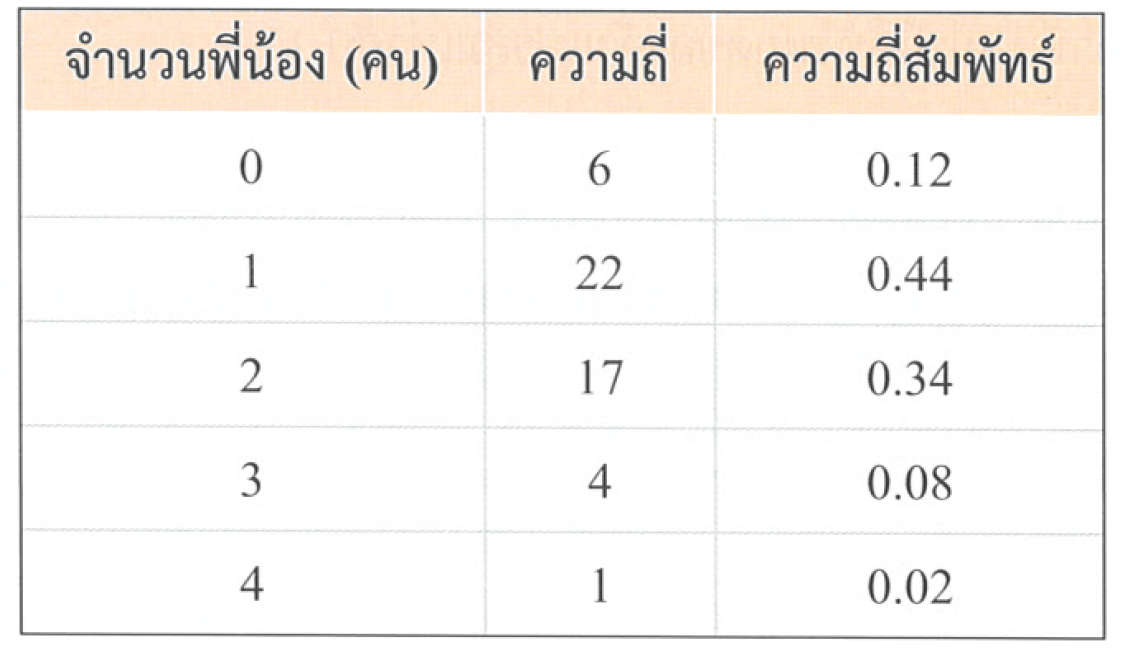
\includegraphics[scale=0.50]{1} 
	\caption{} 
	\label{Figure1} 
\end{figure}
	ถ้าสุ่มนักเรียน $1$ คน จากห้องนี้ และให้ตัวแปรสุ่ม $X$ คือจำนวนพี่น้องของนักเรียนที่สุ่มได้ จงหา ความน่าจะเป็นที่นักเรียนที่สุ่มได้จะมีพี่น้อง $x$ คน เมื่อ $x \in\{0,1,2,3,4\}$
\end{examplebox}

\solution สำหรับ $x \in\{0,1,2,3,4\}$

จะได้ว่า $P(X=x)$ คือความน่าจะเป็นที่นักเรียนที่สุ่มได้จะมี พี่น้อง $x$ คน
\newpage

จากตัวอย่างข้างต้น จะเห็นว่าความน่าจะเป็นของการเกิดค่าแต่ละค่าที่เป็นไปได้ของตัวแปรสุ่ม คือความถี่สัมพัทธ์

โดยทั่วไป สำหรับตัวแปรสุ่ม $X$ ใด ๆ จะได้ $0 \leq P(X=x) \leq 1$ และผลรวมของความน่าจะเป็น ของการเกิดค่าแต่ละค่าที่เป็นไปได้ทั้งหมดของตัวแปรสุ่มเท่ากับ $1$

เมื่อนำความน่าจะเป็นของการเกิดค่าแต่ละค่าที่เป็นไปได้ทั้งหมดของตัวแปรสุ่มมาเขียนแสดงเพื่อ อธิบายลักษณะของตัวแปรสุ่ม จะเรียกว่า \textbf{การแจกแจงความน่าจะเป็น (probability distribution)} โดยอาจเขียนแสดงในรูปตารางหรือกราฟ เช่น จากตัวอย่างข้างต้น สามารถเขียนตารางแสดงการแจกแจงความน่าจะเป็นของตัวแปรสุ่ม $X$ ได้ดังนี้

\begin{figure}[H] 
	\centering 
	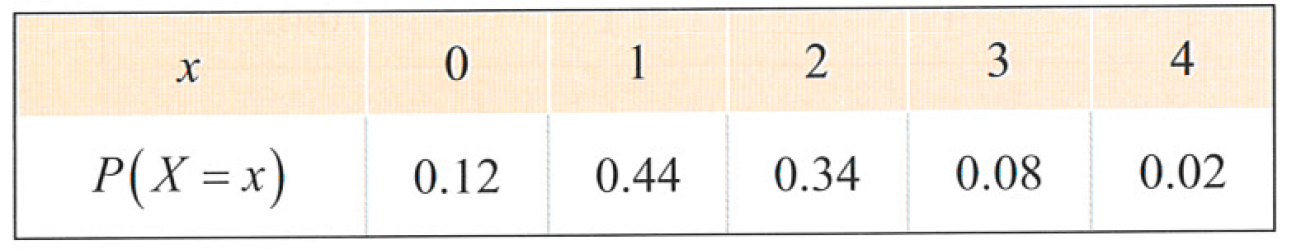
\includegraphics[scale=0.50]{2} 
	\caption{} 
	\label{Figure2} 
\end{figure}

\newpage
\begin{examplebox} \label{example2}
	ให้ตัวแปรสุ่ม $X$ คือจำนวนครั้งที่เหรียญขึ้นหัว จากการโยนเหรียญที่เที่ยงตรง $1$ เหรียญ $3$ ครั้ง จงเขียน แสดงการแจกแจงความน่าจะเป็นของตัวแปรสุ่ม $X$ ในรูปตารางและกราฟ
\end{examplebox}
\solution ให้ $S$ แทนปริภูมิตัวอย่างของการโยนเหรียญที่เที่ยงตรง $1$ เหรียญ $3$ ครั้ง $H$ แทนเหรียญขึ้นหัว\\
และ $T$ แทนเหรียญขึ้นก้อย

\newpage
ได้ตารางแสดงการแจกแจงความน่าจะเป็นของตัวแปรสุ่ม $X$ ได้ดังนี้
\begin{figure}[H] 
	\centering 
	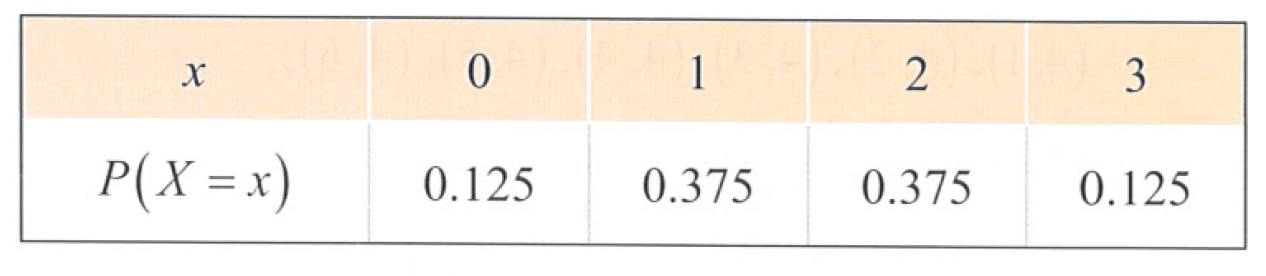
\includegraphics[scale=0.50]{3} 
	\caption{} 
	\label{Figure3} 
\end{figure}
และได้กราฟแสดงการแจกแจงความน่าจะเป็นของตัวแปรสุ่ม $X$ ได้ดังนี้
\begin{figure}[H] 
	\centering 
	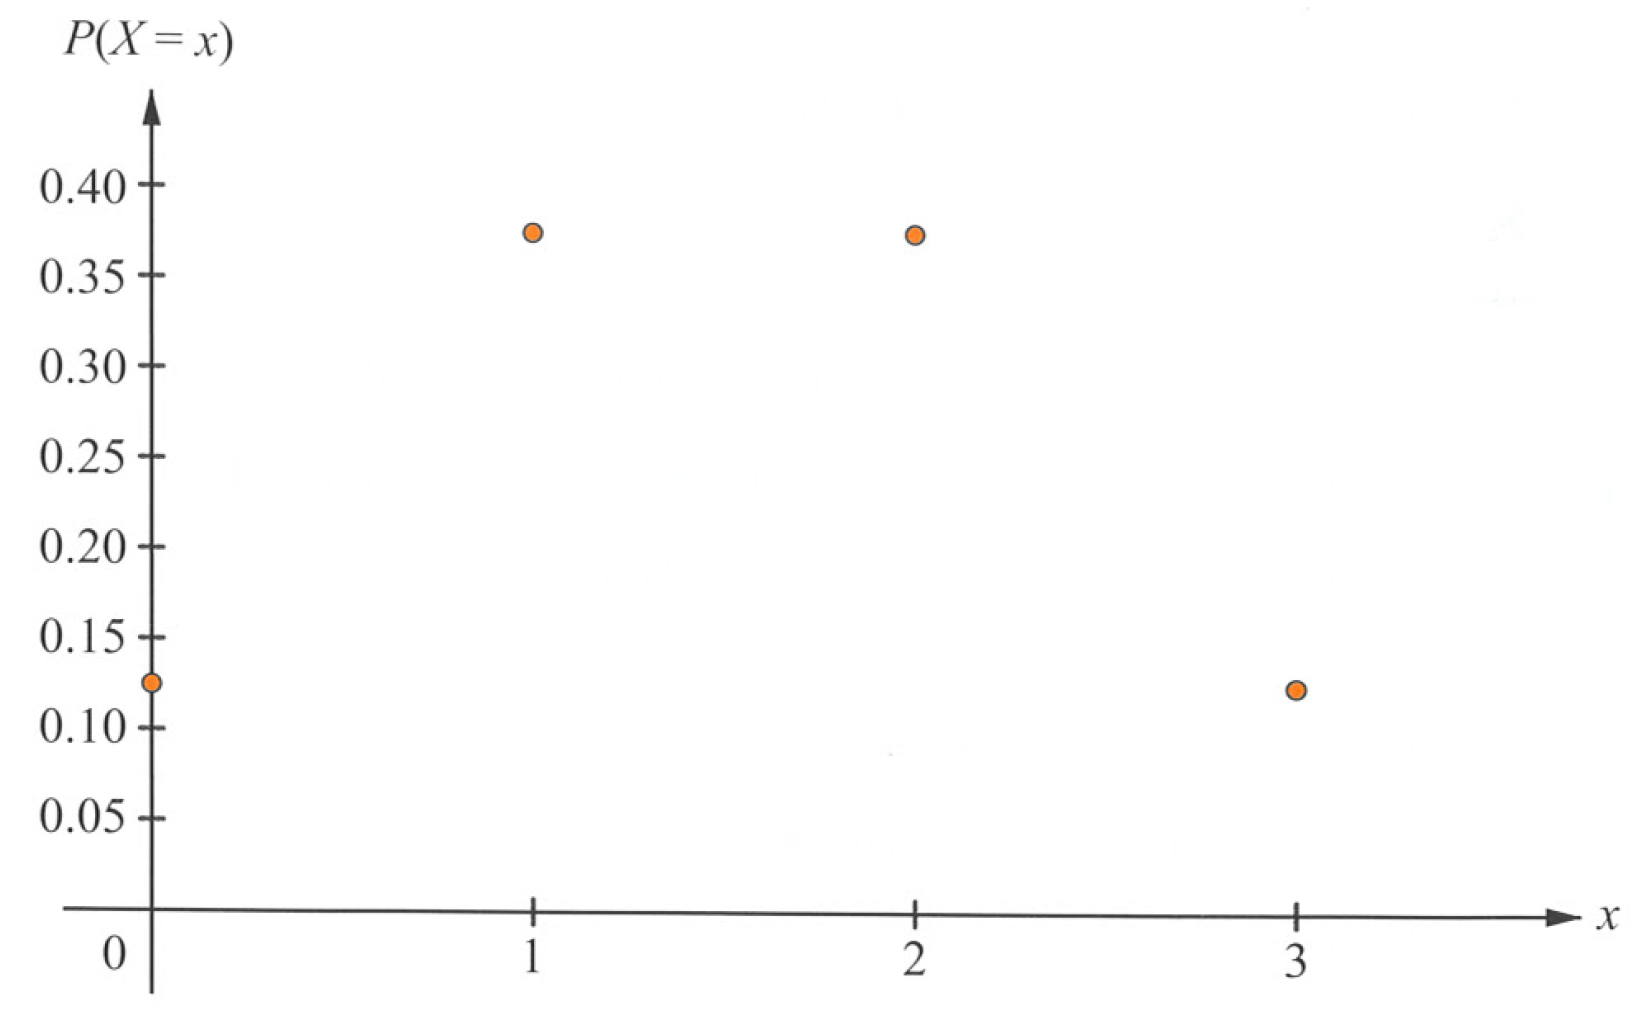
\includegraphics[scale=0.60]{4} 
	\caption{} 
	\label{Figure4} 
\end{figure}

\newpage
\begin{examplebox} \label{example3}
	ให้ตัวแปรสุ่ม $Y$ คือผลบวกของแต้มบนหน้าลูกเต๋า จากการทอดลูกเต๋าที่เที่ยงตรง $2$ ลูก พร้อมกัน $1$ ครั้ง จงเขียนแสดงการแจกแจงความน่าจะเป็นของตัวแปรสุ่ม $Y$ ในรูปตารางและกราฟ
\end{examplebox}
\solution ให้ $S$ แทนปริภูมิตัวอย่างของการทอดลูกเต๋าที่เที่ยงตรง $2$ ลูก พร้อมกัน $1$ ครั้ง

\newpage

ได้ตารางแสดงการแจกแจงความน่าจะเป็นของตัวแปรสุ่ม $X$ ได้ดังนี้
\begin{figure}[H] 
	\centering 
	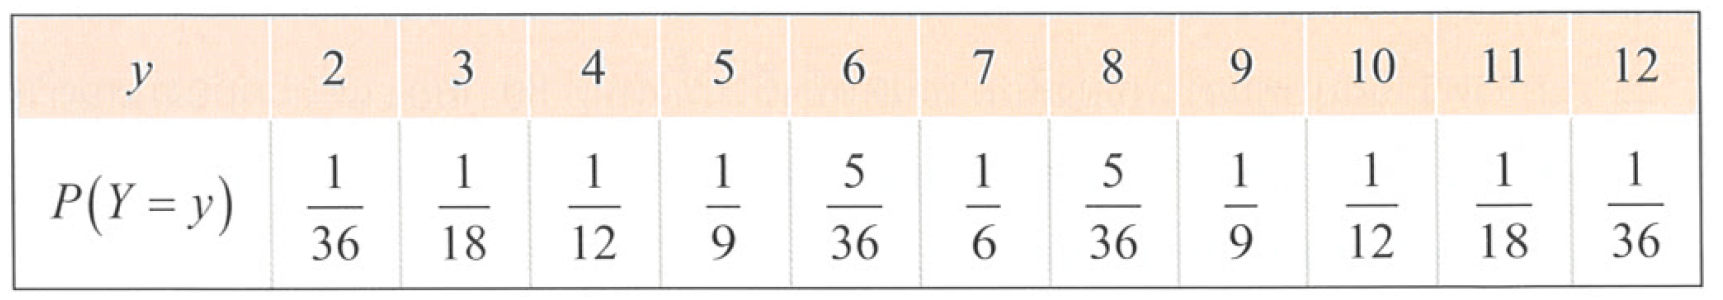
\includegraphics[scale=0.50]{5} 
	\caption{} 
	\label{Figure5} 
\end{figure}
และได้กราฟแสดงการแจกแจงความน่าจะเป็นของตัวแปรสุ่ม $X$ ได้ดังนี้
\begin{figure}[H] 
	\centering 
	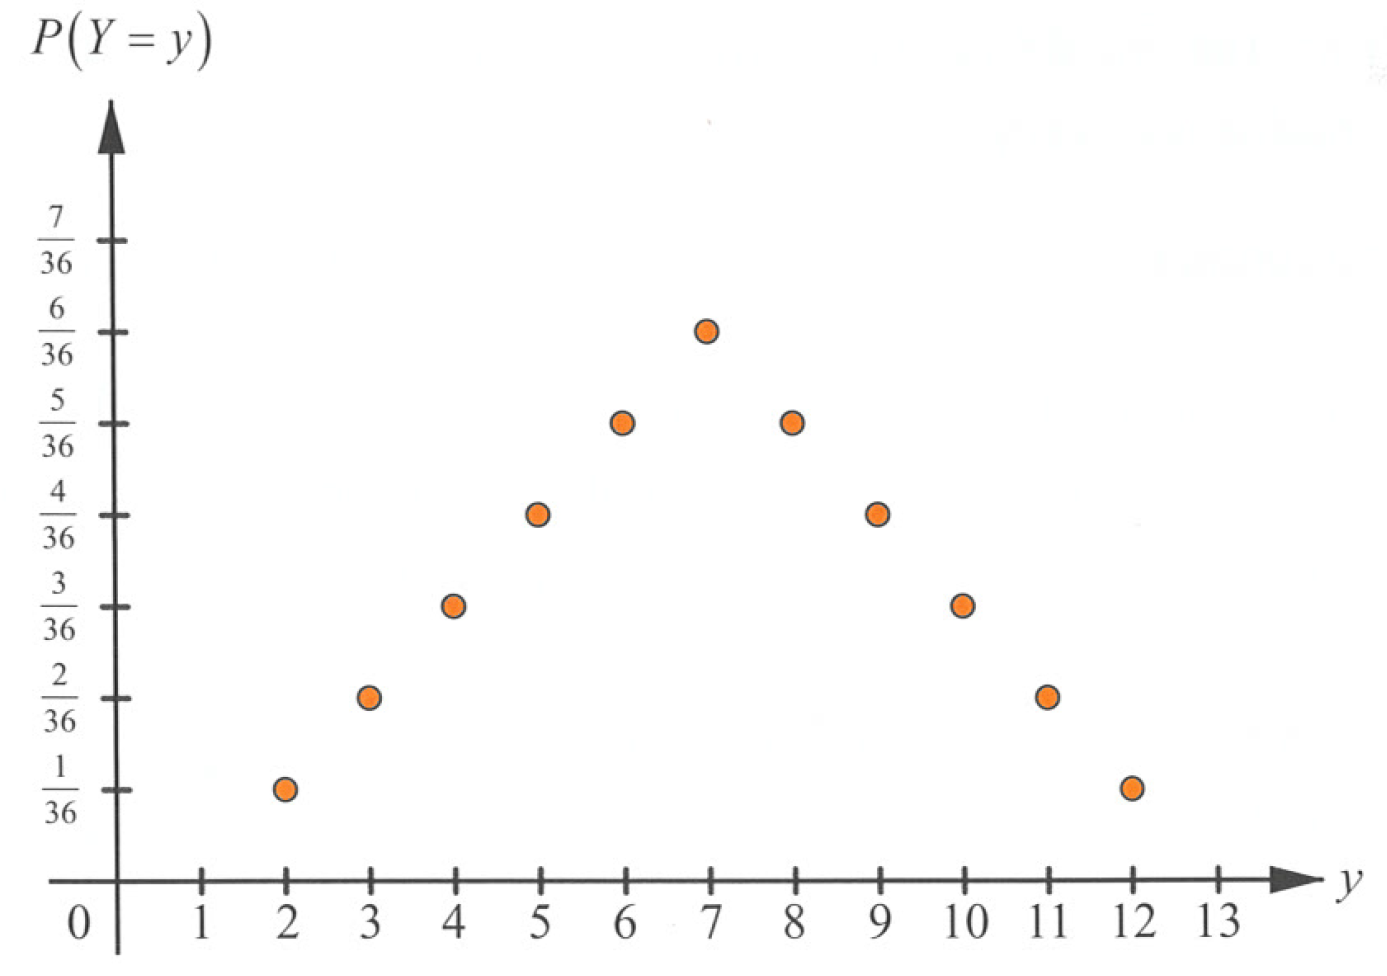
\includegraphics[scale=0.60]{6} 
	\caption{} 
	\label{Figure6} 
\end{figure}
\newpage
\section{ค่าคาดหมายและส่วนเบี่ยงเบนมาตรฐานของตัวแปรสุ่มไม่ต่อเนื่อง}
ต่อไปจะนิยามค่าคาดหมายของตัวแปรสุ่มไม่ต่อเนื่องดังนี้
\begin{definitionbox}
	\textbf{ค่าคาดหมาย (expected value)} ของตัวแปรสุ่มไม่ต่อเนื่อง $X$ เขียนแทนด้วย $\mu_{X}$ นิยามโดย
	
	$$
	\mu_{X}=\sum_{i=1}^{n} x_{i} P\left(X=x_{i}\right)
	$$
	
	เมื่อ $n$ แทนจำนวนค่าที่เป็นไปได้ทั้งหมดของตัวแปรสุ่ม $X$ และ $x_{1}, x_{2}, x_{3}, \ldots, x_{n}$ แทนค่าที่ เป็นไปได้ทั้งหมดของตัวแปรสุ่ม $X$
\end{definitionbox}

\remark ในกรณีที่เซตของค่าที่เป็นไปได้ทั้งหมดของตัวแปรสุ่ม $X$ เป็นเซตอนันต์ จะนิยามให้
\[\mu_{X}=\sum_{i=1}^{\infty} x_{i} P\left(X=x_{i}\right)\] แต่ในที่นี้จะพิจารณาเฉพาะกรณีที่เซตของค่าที่เป็นไปได้ทั้งหมด ของตัวแปรสุ่มเป็นเซตจำกัด

\begin{examplebox}\label{example4}
จงหาค่าคาดหมายของตัวแปรสุ่ม $X$ ที่กำหนดในตัวอย่าง \ref{example1}
\end{examplebox}
\solution จากตัวอย่าง \ref{example1} ตัวแปรสุ่ม $X$ คือจำนวนพี่น้องของนักเรียนที่สุ่มได้

จะได้ว่าค่าที่เป็นไปได้ของตัวแปรสุ่ม $X$ คือ $0,1,2,3$ และ $4$

\newpage
ในบทที่ $3$ นักเรียนทราบแล้วว่าค่าเฉลี่ยเลขคณิตเป็นค่ากลางของข้อมูลที่หาได้จากการหารผลรวมของข้อมูลทั้งหมดด้วยจำนวนข้อมูลที่มี จากตัวอย่างที่ $1$ จะได้ว่าค่าเฉลี่ยเลขคณิตของจำนวนพี่น้องของนักเรียน $50$ คน คือ
\begin{equation*}
	\frac{0(6)+1(22)+2(17)+3(4)+4(1)}{50} = 1.44 \text{ คน}
\end{equation*}
สังเกตว่า
\begin{equation*}
	\frac{0(6)+1(22)+2(17)+3(4)+4(1)}{50} = 0\left(\frac{6}{50}\right)+1\left(\frac{22}{50}\right)+2\left(\frac{17}{50}\right)+3\left(\frac{4}{50}\right)+4\left(\frac{1}{50}\right)
\end{equation*}
และจากตัวอย่าง \ref{example4} จะเห็นว่า
\begin{equation*}
	\mu_{X} = 0\left(\frac{6}{50}\right)+1\left(\frac{22}{50}\right)+2\left(\frac{17}{50}\right)+3\left(\frac{4}{50}\right)+4\left(\frac{1}{50}\right)
\end{equation*}
ดังนั้น ค่าเฉลี่ยเลขคณิตของจำนวนพี่น้องของนักเรียน $50$ คน เท่ากับค่าคาดหมายของตัวแปรสุ่ม $X$ เมื่อตัวแปรสุ่ม $X$ คือจำนวนพี่น้องของนักเรียนที่สุ่มได้

จึงอาจเรียกค่าคาดหมายของตัวแปรสุ่มว่า \textbf{ค่าเฉลี่ย (mean)} ของตัวแปรสุ่ม

\newpage
นอกจากจะสามารถพิจารณาค่าคาดหมายเป็นค่าเฉลี่ยของตัวแปรสุ่มแล้ว ค่าคาดหมายของตัวแปรสุ่ม ยังสามารถใช้ช่วยในการตัดสินใจเกี่ยวกับสถานการณ์ต่าง ๆ ได้ดังตัวอย่างต่อไปนี้
\begin{examplebox}
	ในงานประจำปีของจังหวัดหนึ่งมีเกมวงล้อเสี่ยงโชค โดยมีกติกาว่า ผู้เล่นจะต้องหมุนวงล้อที่มีหมายเลข $1-7$ กำกับไว้ดังรูป ถ้าลูกศรชี้ที่ช่องที่มีหมายเลขที่กำกับเป็นจำนวนคี่ ผู้เล่นจะได้เงินรางวัล $20$ บาท สมมติในการหมุนวงล้อแต่ละครั้งโอกาสที่ลูกศรจะชี้ที่ช่องใดช่องหนึ่งเท่ากัน และในการเล่นเกมวงล้อ เสี่ยงโชคแต่ละครั้ง ผู้เล่นจะต้องจ่ายเงินซื้อตั๋วราคา $10$ บาท จงหาค่าคาดหมายของจำนวนเงินที่ผู้เล่น จะได้รับหรือเสียไป พร้อมทั้งอธิบายความหมาย
	\begin{figure}[H] 
		\centering 
		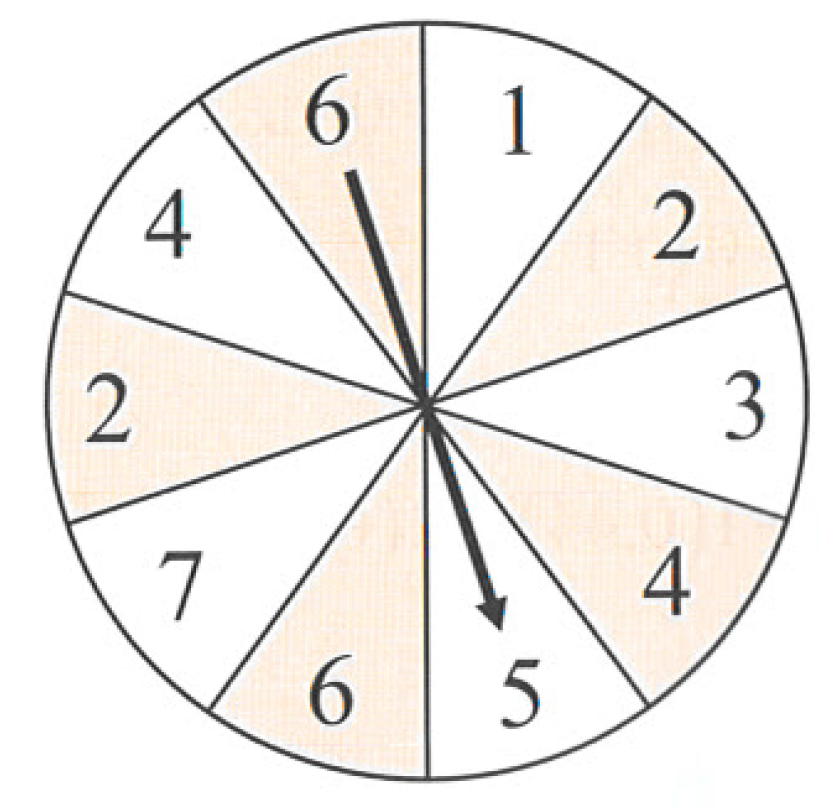
\includegraphics[scale=0.40]{7} 
		\caption{} 
		\label{Figure5} 
	\end{figure}
\end{examplebox}
\solution ให้ตัวแปรสุ่ม $X$ คือกำไร (ขาดทุน) ของผู้เล่นจากการหมุนวงล้อ $1$ ครั้ง เนื่องจากในการหมุนวงล้อ $1$ ครั้ง มีเหตุการณ์ที่เป็นไปได้ $2$ เหตุการณ์ คือ ผู้เล่นได้เงินรางวัล $20$ บาท และผู้เล่นไม่ได้เงินรางวัล

แต่ในการเล่นเกมวงล้อเสี่ยงโชคแต่ละครั้ง ผู้เล่นจะต้องเสียเงิน $10$ บาท จะได้ค่าที่เป็นไปได้ของตัวแปรสุ่ม $X$ คือ $10$ และ $-10$ เนื่องจากผู้เล่นจะได้รับเงินรางวัลก็ต่อเมื่อลูกศรชี้ที่ช่องที่มีหมายเลขที่กำกับเป็นจำนวนคี่ ซึ่งมี $4$ ช่อง จากจำนวนช่องทั้งหมด $10$ ช่อง

ดังนั้น 
\begin{align*}
	P(X=10) &= \frac{4}{10} \\[1ex]
	P(X=-10) &= \frac{6}{10}
\end{align*}

\newpage

นอกจากนี้จะสามารถนิยามส่วนเบี่ยงเบนมาตรฐานของตัวแปรสุ่มเพื่อใช้ในการวัดการกระจายของค่า ที่เป็นไปได้ของตัวแปรสุ่มว่ามีความแตกต่างจากค่าคาดหมายมากหรือน้อยเพียงใด ดังบทนิยามต่อไปนี้
\begin{definitionbox}
	ส่วนเบี่ยงเบนมาตรฐานของตัวแปรสุ่มไม่ต่อเนื่อง $X$ เขียนแทนด้วย $\sigma_{X}$ นิยามโดย
	
	$$
	\sigma_{X}=\sqrt{\sum_{i=1}^{n}\left(x_{i}-\mu_{X}\right)^{2} P\left(X=x_{i}\right)}
	$$
	
	และเรียก $\sigma_{X}^{2}$ ว่า ความแปรปรวนของตัวแปรสุ่มไม่ต่อเนื่อง $X$\\
	เมื่อ $n$ แทนจำนวนค่าที่เป็นไปได้ทั้งหมดของตัวแปรสุ่ม $X$ และ $x_{1}, x_{2}, x_{3}, \ldots, x_{n}$ แทนค่าที่ เป็นไปได้ทั้งหมดของตัวแปรสุ่ม $X$
\end{definitionbox}

\remark ในกรณีที่เซตของค่าที่เป็นไปได้ทั้งหมดของตัวแปรสุ่ม $X$ เป็นเซตอนันต์ จะนิยามให้
\[\sigma_{X}=\sqrt{\sum_{i=1}^{\infty}\left(x_{i}-\mu_{X}\right)^{2} P\left(X=x_{i}\right)}\]
แต่ในที่นี้จะพิจารณาเฉพาะกรณีที่เซตของค่าที่ เป็นไปได้ทั้งหมดของตัวแปรสุ่มเป็นเซตจำกัด
\begin{examplebox}
ให้ตัวแปรสุ่ม $X$ คือจำนวนครั้งที่เหรียญขึ้นหัว จากการโยนเหรียญที่เที่ยงตรง $1$ เหรียญ $3$ ครั้ง จงหา ค่าคาดหมาย ความแปรปรวน และส่วนเบี่ยงเบนมาตรฐานของตัวแปรสุ่ม $X$
\end{examplebox}
\solution จากตัวอย่าง \ref{example2} จะได้ตารางแจกแจงความน่าจะเป็นของตัวแปรสุ่ม $X$ ดังนี้
	\begin{figure}[H] 
	\centering 
	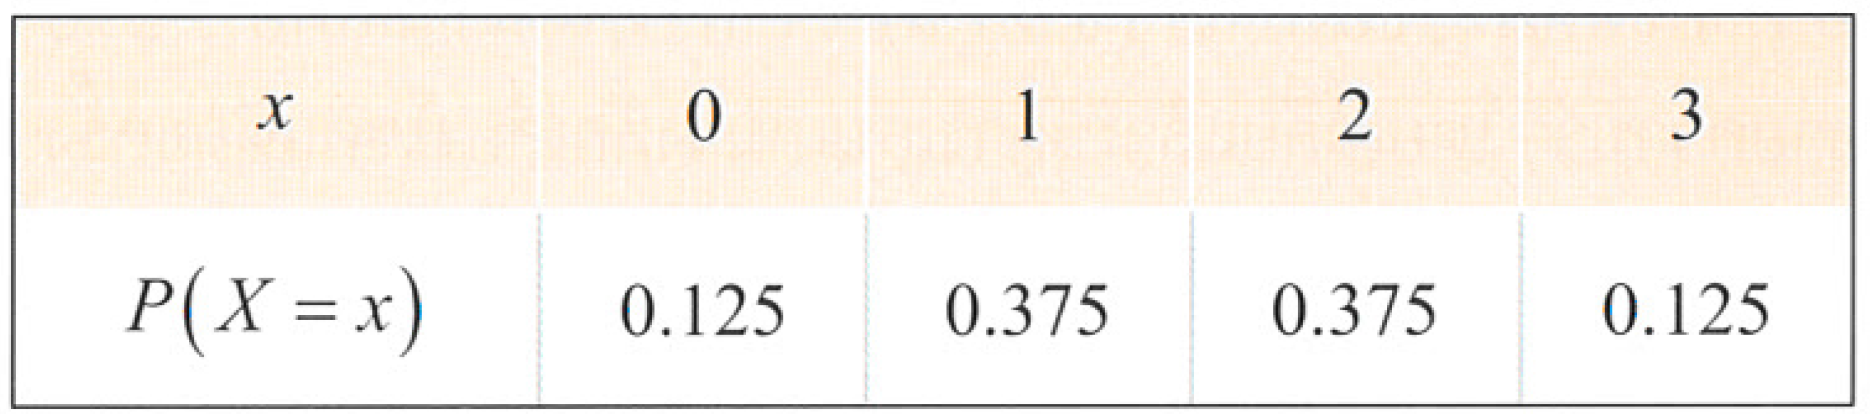
\includegraphics[scale=0.35]{8} 
	\caption{} 
	\label{Figure8} 
\end{figure}

\newpage
\begin{examplebox}
ให้ตัวแปรสุ่ม $Y$ คือผลบวกของแต้มบนหน้าลูกเต๋า จากการทอดลูกเต๋าที่เที่ยงตรง $2$ ลูก พร้อมกัน $1$ ครั้ง จงหาค่าคาดหมาย ความแปรปรวน และส่วนเบี่ยงเบนมาตรฐานของตัวแปรสุ่ม $Y$
\end{examplebox}
\solution จากตัวอย่าง \ref{example3} จะได้ตารางแจกแจงความน่าจะเป็นของตัวแปรสุ่ม $Y$ ดังนี้
	\begin{figure}[H] 
	\centering 
	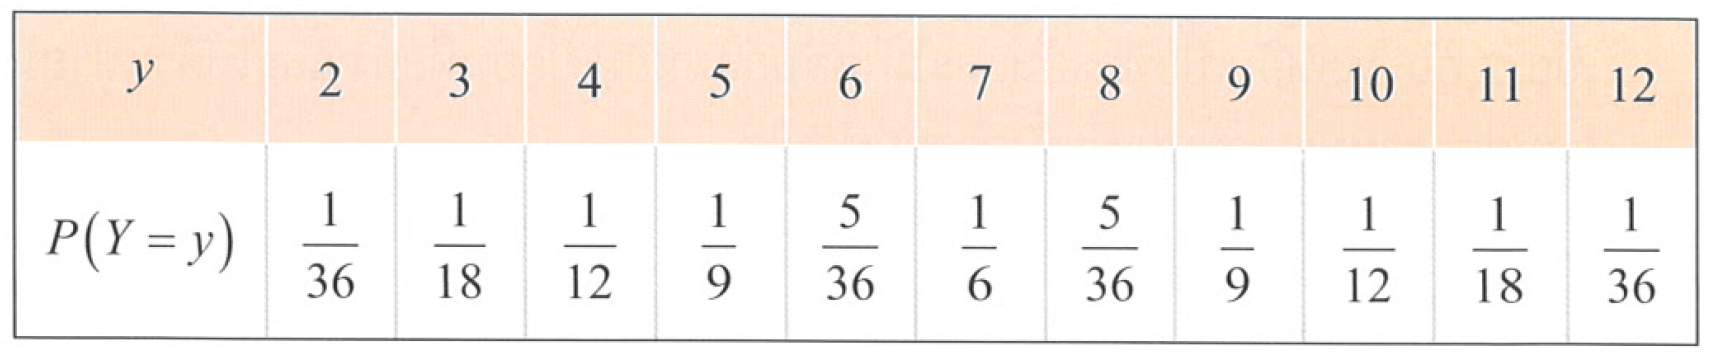
\includegraphics[scale=0.50]{9} 
	\caption{} 
	\label{Figure9} 
\end{figure}

\newpage
\section{การแจกแจงเอกรูปไม่ต่อเนื่อง}
\begin{definitionbox}
ให้ $X$ เป็นตัวแปรสุ่มไม่ต่อเนื่อง ถ้าค่าที่เป็นไปได้ทั้งหมดของ $X$ คือ $x_{1}, x_{2}, x_{3}, \ldots, x_{n}$ แล้ว การแจกแจงความน่าจะเป็นของตัวแปรสุ่ม $X$ เป็น การแจกแจงเอกรูปไม่ต่อเนื่อง (discrete uniform distribution) เมื่อ $P\left(X=x_{i}\right)=\frac{1}{n}$ สำหรับทุก $i \in\{1,2,3, \ldots, n\}$
\end{definitionbox}
จากบทนิยาม จะเห็นว่าการแจกแจงความน่าจะเป็นของตัวแปรสุ่มจะเป็นการแจกแจงเอกรูป ไม่ต่อเนื่อง เมื่อการเกิดค่าแต่ละค่าที่เป็นไปได้ของตัวแปรสุ่มมีความน่าจะเป็นเท่ากัน

\begin{examplebox}
ในการทอดลูกเต๋าที่เที่ยงตรง $1$ ลูก $1$ ครั้ง ให้ตัวแปรสุ่ม $X$ คือแต้มบนหน้าลูกเต๋า จงพิจารณา ว่าการแจกแจงความน่าจะเป็นของตัวแปรสุ่ม $X$ เป็นการแจกแจงเอกรูปไม่ต่อเนื่องหรือไม่ พร้อมทั้งเขียนแสดงการแจกแจงความน่าจะเป็นของตัวแปรสุ่ม $X$ ในรูปตารางและกราฟ
\end{examplebox}
\solution ค่าที่เป็นไปได้ของตัวแปรสุ่ม $X$ คือ $1, 2, 3, 4, 5$ และ $6$

สำหรับ $x \in \{1, 2, 3, 4, 5, 6\}$ จะได้ว่า $P(X=x)$ คือความน่าจะเป็นที่ลูกเต๋าขึ้นแต้ม $x$ เนื่องจากลูกเต๋าเที่ยงตรง จะได้ว่า
\begin{equation*}
	P(X=x) = \frac{1}{6}
\end{equation*}
ดังนั้น การแจกแจงความน่าจะเป็นของตัวแปรสุ่ม $X$ เป็นการแจกแจงเอกรูปไม่ต่อเนื่อง จะได้ตารางแสดงการแจกแจงความน่าจะเป็นของตัวแปรสุ่ม $X$ ดังนี้

	\begin{figure}[H] 
	\centering 
	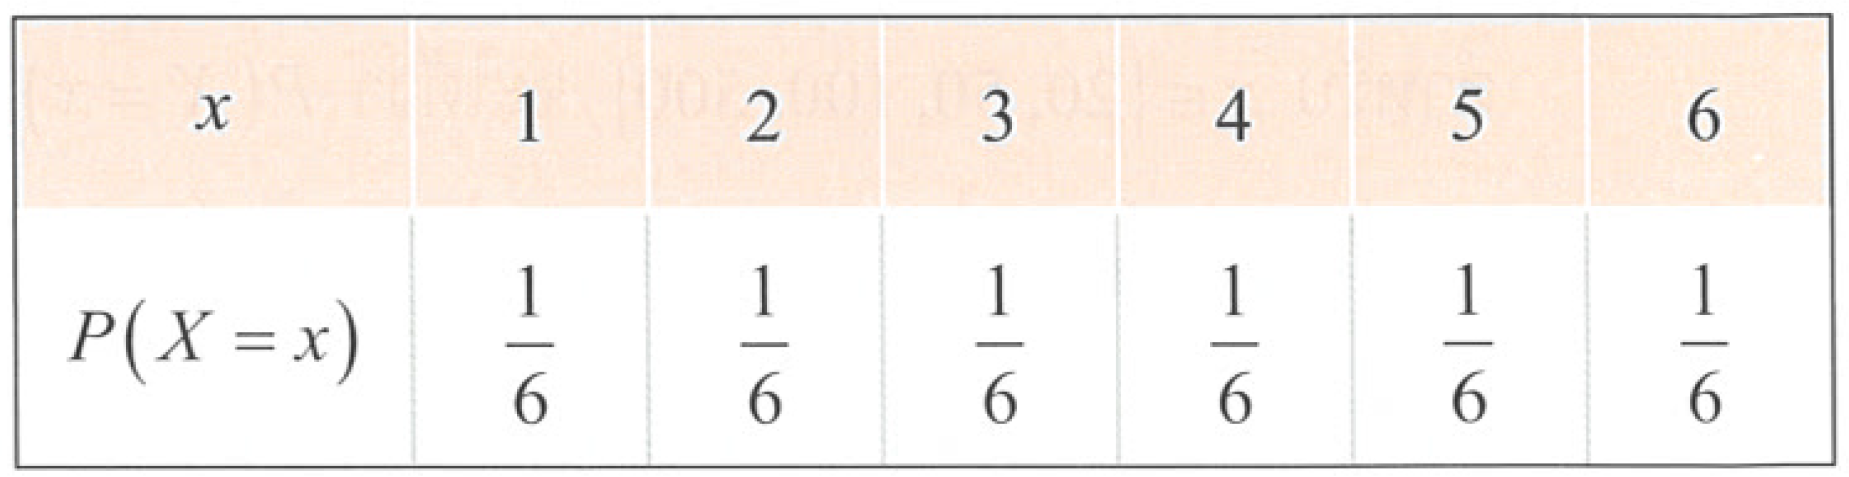
\includegraphics[scale=0.45]{10} 
	\caption{} 
	\label{Figure10} 
\end{figure}
และได้กราฟแสดงการแจกแจงความน่าจะเป็นของตัวแปรสุ่ม $X$ ดังนี้
	\begin{figure}[H] 
	\centering 
	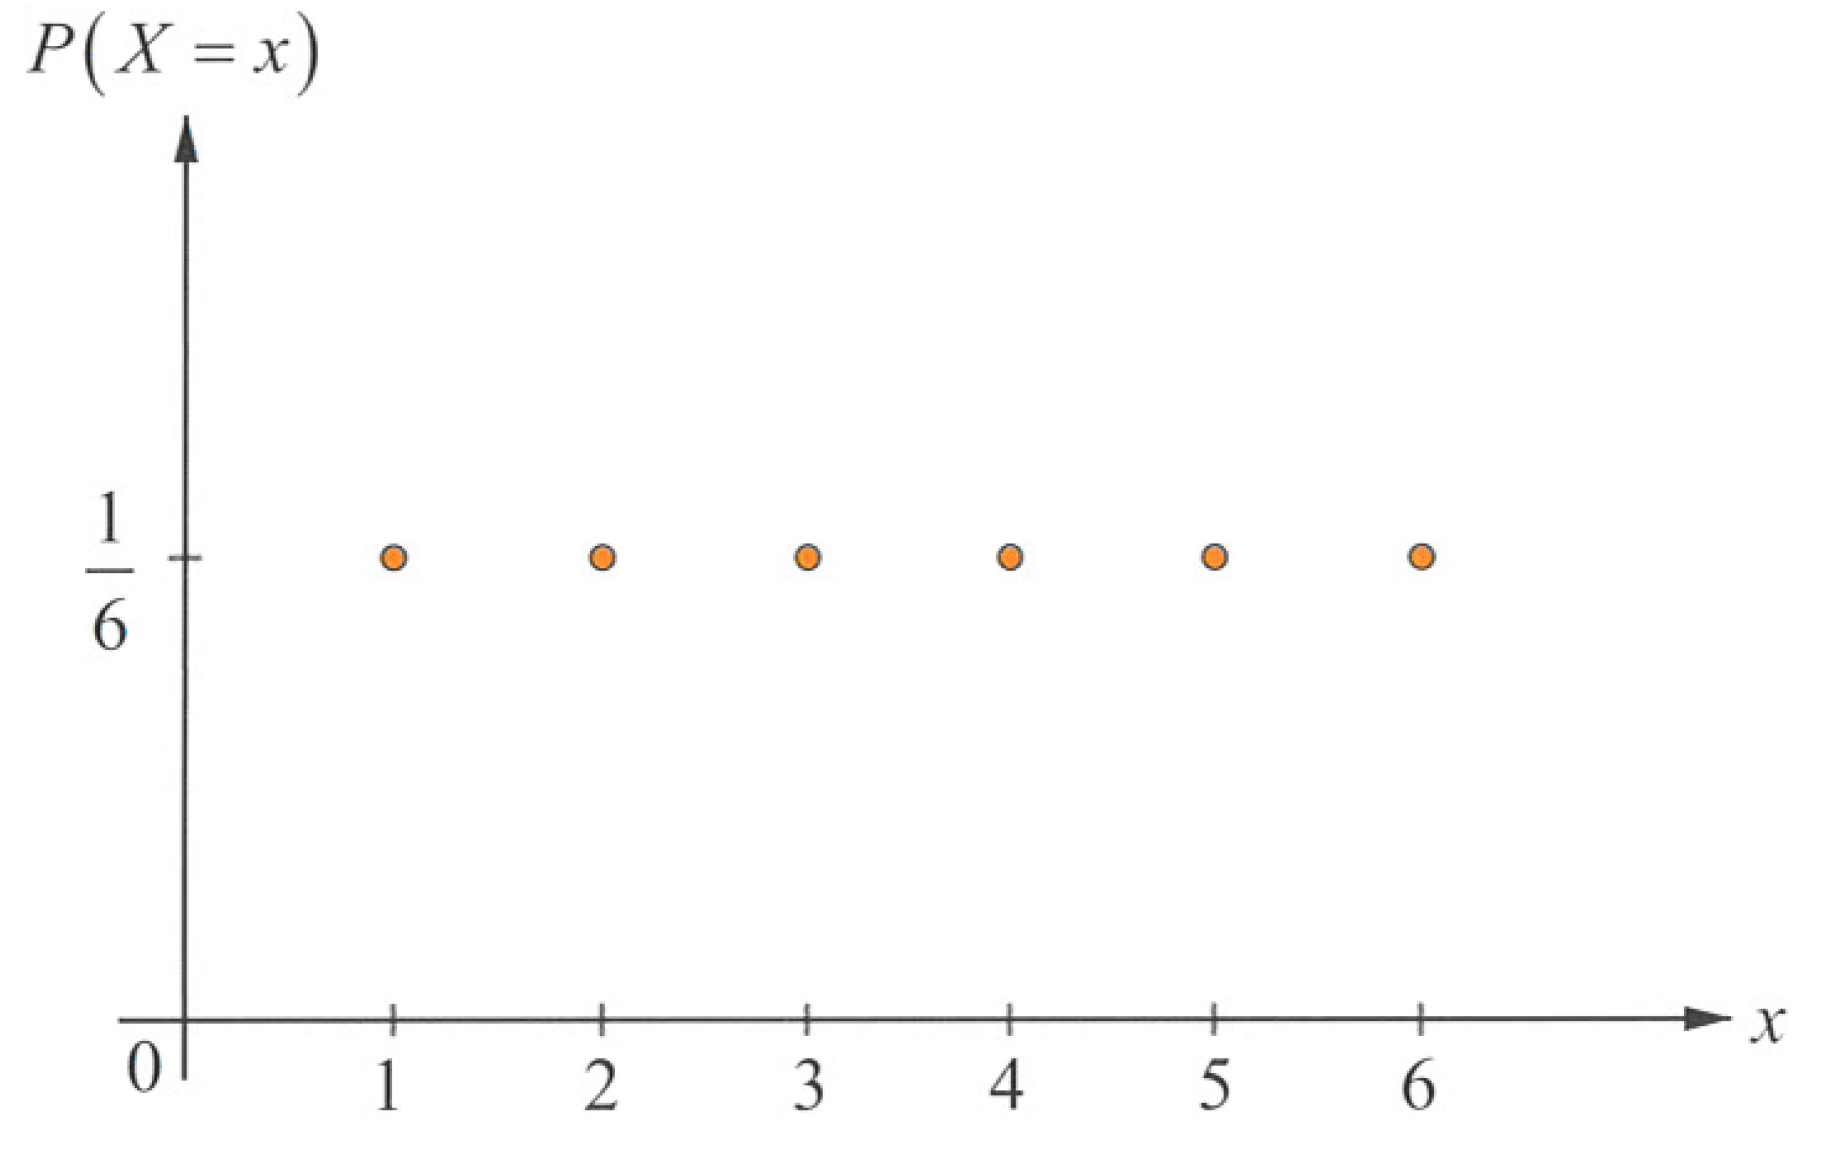
\includegraphics[scale=0.50]{11} 
	\caption{} 
	\label{Figure11} 
\end{figure}
\newpage
\begin{examplebox}
ลูกคิดสุ่มหยิบสลาก $1$ ใบ จากกล่องที่บรรจุสลาก $4$ ใบ แต่ละใบระบุจำนวนเงินรางวัล แตกต่างกันคือ $20, 50, 100$ และ $500$ บาท ให้ตัวแปรสุ่ม $X$ คือจำนวนเงินรางวัลที่ลูกคิด จะได้รับ

\begin{enumerate}
	\item จงพิจารณาว่าการแจกแจงความน่าจะเป็นของตัวแปรสุ่ม $X$ เป็นการแจกแจงเอกรูป ไม่ต่อเนื่องหรือไม่
	\item จงหาค่าคาดหมายของตัวแปรสุ่ม $X$
	\item ถ้าลูกคิดต้องจ่ายเงินซื้อตั๋วราคา $150$ บาท เพื่อหยิบสลาก $1$ ใบ จงพิจารณาว่าถ้าลูกคิด สุ่มหยิบสลากหลาย ๆ ครั้ง โดยเฉลี่ยแล้วลูกคิดได้เปรียบหรือเสียเปรียบ
\end{enumerate}
\end{examplebox}
\solution 

\newpage
\section{การแจกแจงทวินาม}
นักเรียนได้ศึกษาเกี่ยวกับการแจกแจงเอกรูปไม่ต่อเนื่อง ซึ่งเป็นการแจกแจงความน่าจะเป็นของตัวแปรสุ่มอย่างง่าย เนื่องจากการเกิดค่าแต่ละค่าที่เป็นไปได้ของตัวแปรสุ่ม มีความน่าจะเป็นเท่ากัน ซึ่งอาจพบได้ไม่มากนักในชีวิตจริง สำหรับหัวข้อนี้ จะศึกษา เกี่ยวกับการแจกแจงความน่าจะเป็นของตัวแปรสุ่มที่มีลักษณะเฉพาะประเภทหนึ่ง ซึ่งความ น่าจะเป็นของการเกิดค่าแต่ละค่าที่เป็นไปได้ของตัวแปรสุ่มไม่จำเป็นต้องเท่ากัน ดังเช่น ในตัวอย่าง \ref{example2} เมื่อกำหนดให้ตัวแปรสุ่ม $X$ คือจำนวนครั้งที่เหรียญขึ้นหัว จากการโยนเหรียญ ที่เที่ยงตรง $1$ เหรียญ $3$ ครั้ง จะได้ว่า $X$ เป็นตัวแปรสุ่มไม่ต่อเนื่อง สังเกตว่าในแต่ละครั้งที่ โยนเหรียญจะมีผลลัพธ์ที่เป็นไปได้ $2$ แบบ คือ เหรียญขึ้นหัวหรือก้อย แต่จากการกำหนด ตัวแปรสุ่ม $X$ จะเห็นว่าสนใจจำนวนครั้งที่เหรียญขึ้นหัว จึงอาจพิจารณาว่าในการโยนเหรียญ แต่ละครั้ง ถ้าเหรียญขึ้นหัวคือ สำเร็จ แต่ถ้าเหรียญขึ้นก้อยคือ ไม่สำเร็จ ดังนั้น สามารถพิจารณา ว่าตัวแปรสุ่ม $X$ คือ จำนวนครั้งของการเกิดผลสำเร็จจากการโยนเหรียญที่เที่ยงตรง $1$ เหรียญ เป็นจำนวน $3$ ครั้ง เช่น เหตุการณ์ที่ $X=1$ ซึ่งคือ $\{HTT, THT, TTH\}$ หมายความว่า แต่ละสมาชิก ในเหตุการณ์นี้เกิดผลสำเร็จ $1$ ครั้ง (เหรียญขึ้นหัว $1$ ครั้ง) และไม่เกิดผลสำเร็จ $2$ ครั้ง (เหรียญขึ้น ก้อย $2$ ครั้ง) นอกจากนี้จะเห็นว่าผลที่ได้จากการโยนเหรียญในครั้งก่อนหน้าไม่ส่งผลต่อการ โยนเหรียญครั้งต่อไปและความน่าจะเป็นที่จะเกิดผลสำเร็จในการโยนเหรียญแต่ละครั้งเท่ากัน คือ $\dfrac{1}{2}$

การแจกแจงความน่าจะเป็นของตัวแปรสุ่มในตัวอย่างข้างต้น เรียกว่า การแจกแจงทวินาม ซึ่งมีบทนิยามดังนี้
\begin{definitionbox}
	\textbf{การแจกแจงทวินาม (binomial distribution)} คือ การแจกแจงความน่าจะเป็นของ ตัวแปรสุ่ม $X$ ซึ่งคือจำนวนครั้งของการเกิดผลสำเร็จจากการทดลองสุ่ม $n$ ครั้ง ที่เป็น อิสระกัน โดยในแต่ละครั้งมีโอกาสเกิดผลสำเร็จด้วยความน่าจะเป็นเท่ากับ $p$ และ ไม่เกิดผลสำเร็จด้วยความน่าจะเป็นเท่ากับ $1-p$
\end{definitionbox}
\remark 
\begin{enumerate}
	\item เรียก $n$ และ $p$ ว่า \textbf{พารามิเตอร์ของการแจกแจงทวินาม} และเขียนสัญลักษณ์ $X \sim B(n, p)$ เพื่อแสดงว่าการแจกแจงความน่าจะเป็นของตัวแปรสุ่ม $X$ เป็นการแจกแจงทวินามที่มี $n$ และ $p$ เป็นพารามิเตอร์
	\item การทดลองสุ่ม $1$ ครั้ง ที่มีผลลัพธ์ที่เป็นไปได้ $2$ แบบ คือ สำเร็จหรือไม่สำเร็จ เรียกว่า \textbf{การลองแบร์นูลลี (Bernoulli trial)} เช่น การโยนเหรียญ $1$ เหรียญ $1$ ครั้ง
\end{enumerate}

จากบทนิยามข้างต้น สรุปได้ว่า การแจกแจงทวินามคือการแจกแจงความน่าจะเป็นของตัวแปรสุ่ม ไม่ต่อเนื่องที่มีลักษณะดังต่อไปนี้

\begin{enumerate}
	\item เกิดจากการทดลองสุ่มจำนวน $n$ ครั้งที่เป็นอิสระกัน กล่าวคือ ผลที่ได้จากการทดลองสุ่ม ในครั้งก่อนหน้าไม่ส่งผลต่อการทดลองสุ่มในครั้งต่อ ๆ ไป
	\item การทดลองสุ่มแต่ละครั้งมีผลลัพธ์ที่เป็นไปได้เพียง 2 แบบ คือ สำเร็จหรือไม่สำเร็จ
	\item ความน่าจะเป็นที่จะเกิดผลสำเร็จในการทดลองสุ่มแต่ละครั้งเท่ากัน ให้เป็น $p$ เมื่อ $0<p<1$ และจะได้ว่าความน่าจะเป็นที่จะไม่เกิดผลสำเร็จในการทดลองสุ่มแต่ละครั้งเป็น $1-p$
\end{enumerate}

ทฤษฎีบทต่อไปนี้ใช้ในการหาความน่าจะเป็น ค่าคาดหมาย และส่วนเบี่ยงเบนมาตรฐานของ ตัวแปรสุ่มที่มีการแจกแจงความน่าจะเป็นเป็นการแจกแจงทวินาม โดยในที่นี้จะขอละการพิสูจน์

\begin{theorembox} \label{theorem1}
	ถ้าการแจกแจงความน่าจะเป็นของตัวแปรสุ่ม $X$ เป็นการแจกแจงทวินาม จะได้ว่า
	
	\begin{enumerate}
		\item $P(X=x)=\displaystyle\binom{n}{x} p^{x}(1-p)^{n-x}$ สำหรับทุก $x \in\{0,1,2, \ldots, n\}$
		\item $\mu_{X}=n p$
		\item $\sigma_{X}=\sqrt{n p(1-p)}$
	\end{enumerate}
	
	เมื่อ $n$ แทนจำนวนครั้งของการทดลองสุ่ม และ $p$ แทนความน่าจะเป็นที่จะเกิดผลสำเร็จ ในการทดลองสุ่มแต่ละครั้ง
\end{theorembox}
\remark จากทฤษฎีบท \ref{theorem1} ข้อ 1 และทฤษฎีบททวินาม จะได้ว่า

$$
\sum_{x=0}^{n} P(X=x)=\sum_{x=0}^{n}\binom{n}{x} p^{x}(1-p)^{n-x}=(p+(1-p))^{n}=1
$$

\newpage
\begin{examplebox}
ให้ตัวแปรสุ่ม $X$ คือจำนวนครั้งที่ลูกเต๋าขึ้นแต้ม $5$ จากการทอดลูกเต๋าที่เที่ยงตรง $1$ ลูก $7$ ครั้ง
\begin{enumerate}
	\item จงพิจารณาว่าการแจกแจงความน่าจะเป็นของตัวแปรสุ่ม $X$ เป็นการแจกแจงทวินามหรือไม่
	\item จงหาความน่าจะเป็นที่ลูกเต๋าขึ้นแต้ม $5$ เป็นจำนวน $5$ ครั้ง
	\item จงเขียนแสดงการแจกแจงความน่าจะเป็นของตัวแปรสุ่ม $X$ ในรูปตารางและกราฟ
	\item จงหาค่าคาดหมายและความแปรปรวนของตัวแปรสุ่ม $X$
\end{enumerate}
\end{examplebox}
\solution 
\begin{enumerate}[label=\arabic*), leftmargin=2.5em]
	\item เนื่องจากตัวแปรสุ่ม $X$ มีลักษณะดังต่อไปนี้
	\begin{enumerate}[label=\arabic*., leftmargin=2.5em]
	\item เกิดจากการทดลองสุ่ม (การทอดลูกเต๋าที่เที่ยงตรง $1$ ลูก) จำนวน $7$ ครั้ง ที่เป็น อิสระกัน
	\item การทดลองสุ่มแต่ละครั้งเกิดผลลัพธ์ได้เพียง $2$ แบบ คือ สำเร็จ (ลูกเต๋าขึ้นแต้ม $5$) หรือไม่สำเร็จ (ลูกเต๋าไม่ขึ้นแต้ม $5$)
	\item ความน่าจะเป็นที่ลูกเต๋าขึ้นแต้ม $5$ ในการทอดลูกเต๋าที่เที่ยงตรงแต่ละครั้งเท่ากัน โดยเท่ากับ $\dfrac{1}{6}$ และความน่าจะเป็นที่ลูกเต๋าไม่ขึ้นแต้ม $5$ ในการทอดลูกเต๋า ที่เที่ยงตรงแต่ละครั้งเป็น $1-\dfrac{1}{6}=\dfrac{5}{6}$\\
	ดังนั้น การแจกแจงความน่าจะเป็นของตัวแปรสุ่ม $X$ เป็นการแจกแจงทวินาม
	\end{enumerate}
\end{enumerate}
\newpage
จะได้ตารางแสดงการแจกแจงความน่าจะเป็นของตัวแปรสุ่ม $X$ ดังนี้
\begin{figure}[H] 
	\centering 
	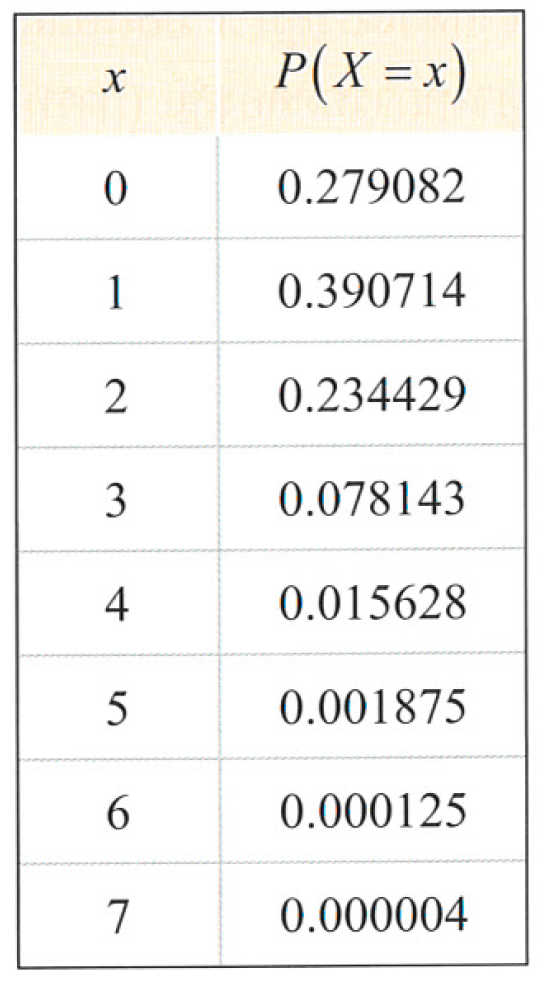
\includegraphics[scale=0.50]{12} 
	\caption{} 
	\label{Figure12} 
\end{figure}
และได้กราฟแสดงการแจกแจงความน่าจะเป็นของตัวแปรสุ่ม $X$ ดังนี้
\begin{figure}[H] 
	\centering 
	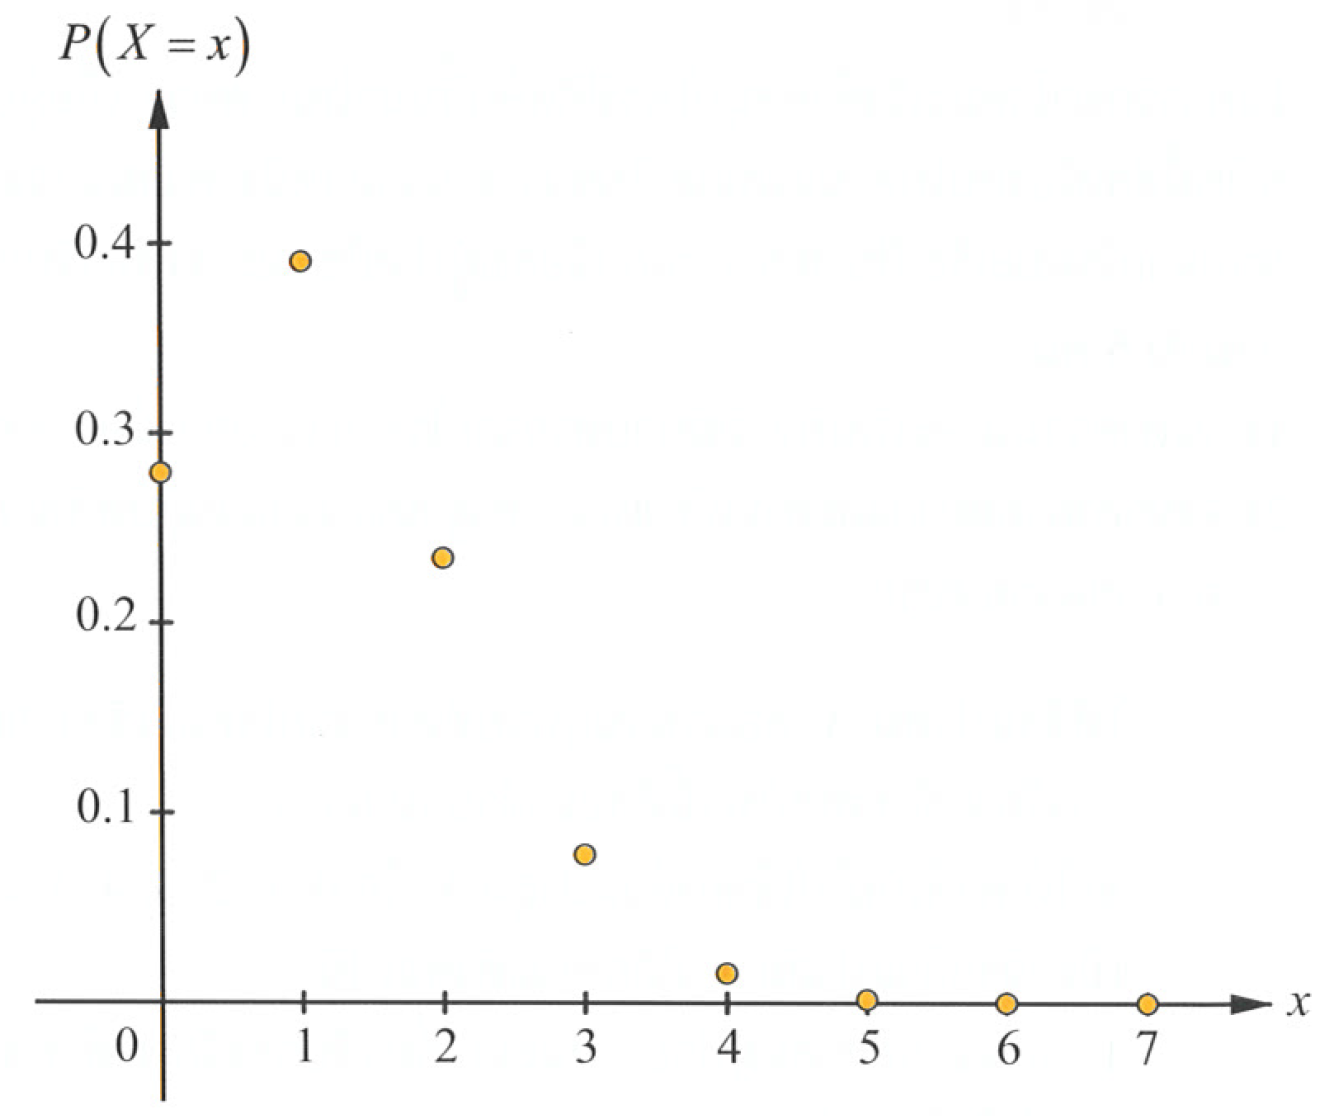
\includegraphics[scale=0.55]{13} 
	\caption{} 
	\label{Figure13} 
\end{figure}
\newpage
\newpage
\begin{examplebox}
ในการรักษาโรคมะเร็งด้วยสมุนไพรที่คิดค้นขึ้นมาใหม่พบว่า เมื่อผู้ป่วยรับประทานสมุนไพร ชนิดนี้ต่อเนื่องกันไปตามแพทย์สั่งในช่วงระยะเวลาหนึ่ง ความน่าจะเป็นที่ผู้ป่วยแต่ละคนจะ หายจากโรคมะเร็งเป็น $0.5$ ถ้านักวิจัยสุ่มผู้ป่วยโรคมะเร็งที่มารับการรักษาด้วยสมุนไพรนี้ จำนวน $6$ คน
\begin{enumerate}[label=\arabic*), leftmargin=2.5em]
	\item จงหาความน่าจะเป็นที่จะมีผู้ป่วยหายจากโรคมะเร็งอย่างน้อย $3$ คน
	\item จงหาค่าคาดหมายและส่วนเบี่ยงเบนมาตรฐานของจำนวนผู้ป่วยที่หายจากโรคมะเร็ง พร้อมทั้ง อธิบายความหมาย
\end{enumerate}
\end{examplebox}
\solution ให้ตัวแปรสุ่ม $X$ คือจำนวนผู้ป่วยที่หายจากโรคมะเร็งจากผู้ป่วยโรคมะเร็งที่มารับ การรักษาด้วยสมุนไพรนี้ที่สุ่มมาจำนวน $6$ คน จะได้ ค่าที่เป็นไปได้ของตัวแปรสุ่ม $X$ คือ $0,1,2,3,4,5$ และ $6$ เนื่องจากตัวแปรสุ่ม $X$ มีลักษณะดังต่อไปนี้
\begin{enumerate}
	\item เกิดจากการสุ่มผู้ป่วยโรคมะเร็งที่มารับการรักษาด้วยสมุนไพรนี้จำนวน $6$ คน ที่เป็นอิสระกัน
	\item การทดลองสุ่มแต่ละครั้งเกิดผลลัพธ์ได้เพียง $2$ แบบ คือ สำเร็จ (ผู้ป่วยที่สุ่มมา หายจากโรคมะเร็ง) หรือไม่สำเร็จ (ผู้ป่วยที่สุ่มมาไม่หายจากโรคมะเร็ง)
	\item ความน่าจะเป็นที่ผู้ป่วยแต่ละคนจะหายจากโรคมะเร็งเท่ากัน โดยเท่ากับ $0.5$ และความน่าจะเป็นที่ผู้ป่วยแต่ละคนจะไม่หายจากโรคมะเร็งเป็น $1-0.5=0.5$ จะเห็นว่าการแจกแจงความน่าจะเป็นของตัวแปรสุ่ม $X$ เป็นการแจกแจงทวินาม
\end{enumerate}

\newpage
\begin{examplebox}
จากข้อมูลเกี่ยวกับคุณภาพของสินค้าซึ่งเก็บรวบรวมมาในอดีตทำให้ทราบว่า ความน่าจะเป็น ที่สินค้าแต่ละชิ้นจะชำรุดเป็น $0.05$ และในกระบวนการตรวจสอบคุณภาพสินค้าของโรงงาน มีหลักการคือพนักงานจะสุ่มสินค้าจำนวน $5$ ชิ้น จากแต่ละกล่องเพื่อตรวจสอบคุณภาพ ถ้าตรวจพบสินค้าชำรุดไม่เกิน $1$ ชิ้น สินค้ากล่องนั้นจะผ่านการตรวจสอบคุณภาพ
\begin{enumerate}[label=\arabic*), leftmargin=2.5em]
	\item จงหาความน่าจะเป็นที่สินค้าแต่ละกล่องที่ส่งมาตรวจสอบจะผ่านการตรวจสอบคุณภาพ
	\item ในการผลิตสินค้าครั้งหนึ่ง ฝ่ายผลิตของโรงงานส่งสินค้ามาให้พนักงานตรวจสอบคุณภาพ จำนวน $100$ กล่อง จะมีสินค้าที่ผ่านการตรวจสอบคุณภาพกี่กล่อง
\end{enumerate}
\end{examplebox}
\solution ให้ตัวแปรสุ่ม $X$ คือจำนวนสินค้าที่ชำรุด เมื่อสุ่มสินค้า $5$ ชิ้น จากแต่ละกล่อง จะได้ ค่าที่เป็นไปได้ของตัวแปรสุ่ม $X$ คือ $0,1,2,3,4$ และ $5$ เนื่องจากตัวแปรสุ่ม $X$ มีลักษณะดังต่อไปนี้
\begin{enumerate}[label=\arabic*., leftmargin=2.5em]
	\item เกิดจากการสุ่มสินค้าจากแต่ละกล่องจำนวน $5$ ครั้ง ที่เป็นอิสระกัน
	\item การทดลองสุ่มแต่ละครั้งเกิดผลลัพธ์ได้เพียง $2$ แบบ คือ สำเร็จ (สินค้าที่สุ่มมา ชำรุด) หรือไม่สำเร็จ (สินค้าที่สุ่มมาไม่ชำรุด)
	\item ความน่าจะเป็นที่สินค้าชำรุดเมื่อสุ่มสินค้าแต่ละครั้งเท่ากัน โดยเท่ากับ $0.05$ และความน่าจะเป็นที่สินค้าไม่ชำรุดเมื่อสุ่มสินค้าแต่ละครั้งเป็น $1-0.05=0.95$ จะเห็นว่าการแจกแจงความน่าจะเป็นของตัวแปรสุ่ม $X$ เป็นการแจกแจงทวินาม
\end{enumerate}

\newpage
\section{การแจกแจงความน่าจะเป็นของตัวแปรสุ่มต่อเนื่อง}
ในกรณีที่ตัวแปรสุ่มที่สนใจเป็นตัวแปรสุ่มต่อเนื่อง เช่น ระยะเวลาที่ลูกค้าใช้บริการในห้างสรรพสินค้า แห่งหนึ่ง น้ำหนักของผู้ป่วยที่เข้ารับการรักษาที่โรงพยาบาลแห่งหนึ่ง เนื่องจากตัวแปรสุ่มต่อเนื่อง มีเซตของค่าที่เป็นไปได้ทั้งหมดเป็นช่วงซึ่งเป็นสับเซตของ $\mathbb{R}$ ซึ่งมีสมาชิกเป็นจำนวนอนันต์ จึงไม่เหมาะ กับการเขียนแสดงการแจกแจงความน่าจะเป็นในรูปตาราง แต่จะใช้ \textbf{เส้นโค้งความหนาแน่น (density curve)} ในการเขียนแสดงการแจกแจงความน่าจะเป็น โดยความน่าจะเป็นที่ตัวแปรสุ่มจะมีค่าอยู่ใน ช่วงใดช่วงหนึ่งจะเท่ากับพื้นที่ที่ปิดล้อมด้วยเส้นโค้งความหนาแน่นกับแกน $X$ ในช่วงนั้น จะเรียกพื้นที่ บริเวณดังกล่าวว่า \textbf{พื้นที่ใต้เส้นโค้งความหนาแน่น}
เส้นโค้งความหนาแน่นเป็นกราฟของฟังก์ชัน $y=f(x)$ โดยที่ $x$ แทนค่าที่เป็นไปได้ของตัวแปรสุ่ม จะเรียกฟังก์ชันนี้ว่า \textbf{ฟังก์ชันความหนาแน่นความน่าจะเป็น (probability density function)}

\remark $f(x)$ เป็นฟังก์ชันความหนาแน่นความน่าจะเป็นของตัวแปรสุ่ม $X$ ก็ต่อเมื่อ

\begin{enumerate}[label=\arabic*., leftmargin=2.5em]
	\item $f(x) \geq 0$ สำหรับทุก $x$ ที่เป็นค่าที่เป็นไปได้ของตัวแปรสุ่ม $X$
	\item พื้นที่ใต้เส้นโค้งความหนาแน่นทั้งหมดจะเท่ากับ $1$
\end{enumerate}

พิจารณาเส้นโค้งความหนาแน่นของตัวแปรสุ่ม $X$ ดังรูป
\begin{figure}[H] 
	\centering 
	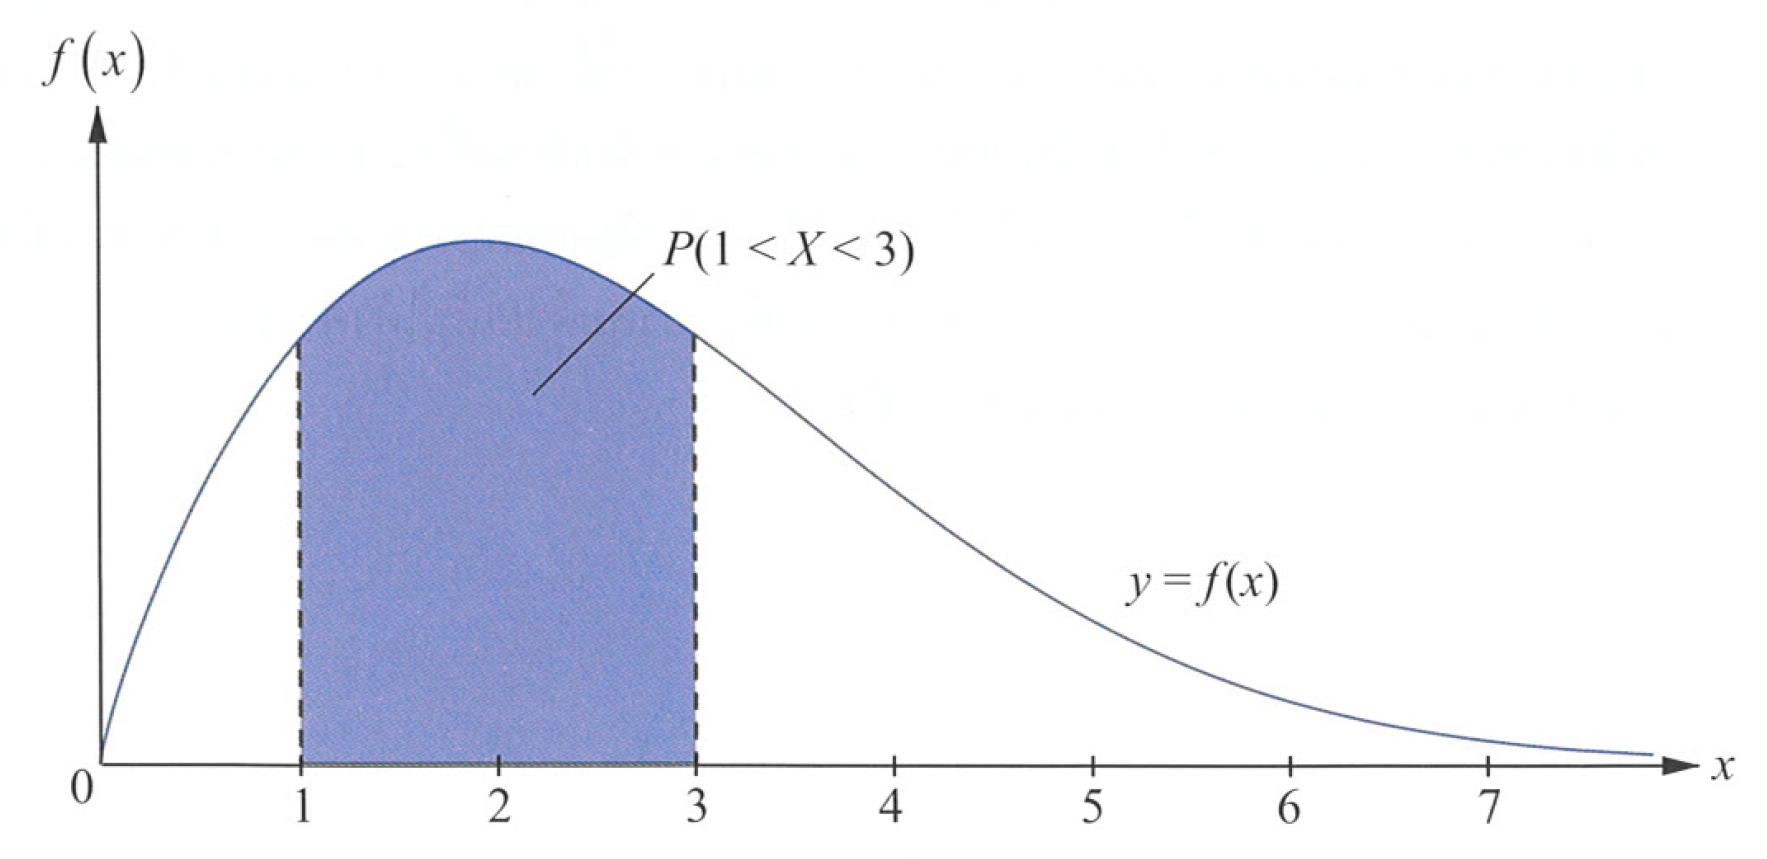
\includegraphics[scale=0.50]{14} 
	\caption{} 
	\label{Figure14} 
\end{figure}

จากรูป สามารถหาความน่าจะเป็นที่ตัวแปรสุ่มจะมีค่าอยู่ในช่วงที่สนใจได้จากการหาพื้นที่ใต้เส้นโค้ง $y=f(x)$ ในช่วงดังกล่าว เช่น ความน่าจะเป็นที่ตัวแปรสุ่ม $X$ มีค่ามากกว่า $1$ แต่น้อยกว่า $3$ จะเท่ากับ พื้นที่ส่วนที่แรเงา นั่นคือ $P(1<X<3)=\displaystyle\int_{1}^{3} f(x) dx$

ดังนั้น ถ้าทราบฟังก์ชันความหนาแน่นความน่าจะเป็น แล้วจะสามารถหาความน่าจะเป็นที่ตัวแปรสุ่ม จะมีค่าอยู่ในช่วงใดช่วงหนึ่งได้โดยการหาปริพันธ์จำกัดเขตของฟังก์ชันในช่วงดังกล่าว

ถ้าให้ $X$ เป็นตัวแปรสุ่มต่อเนื่อง และ $a$ เป็นค่าที่เป็นไปได้ของ $X$ จะได้ว่า $P(X=a)=0$ เนื่องจาก พื้นที่ใต้เส้นโค้งความหนาแน่นจาก $a$ ถึง $a$ เท่ากับศูนย์ ดังนั้น สำหรับตัวแปรสุ่มต่อเนื่อง จะไม่พิจารณา ความน่าจะเป็นของการเกิดค่าของตัวแปรสุ่มค่าใดค่าหนึ่ง แต่จะสนใจเฉพาะความน่าจะเป็นที่ตัวแปร สุ่มจะมีค่าอยู่ในช่วงใดช่วงหนึ่ง โดยความน่าจะเป็นที่ตัวแปรสุ่มจะมีค่าอยู่ในช่วงปิด $[a, b]$ จะเท่ากับ ความน่าจะเป็นที่ตัวแปรสุ่มจะมีค่าอยู่ในช่วงเปิด $(a, b)$ นั่นคือ $P(a \leq X \leq b)=P(a<X<b)$ เมื่อ $a$ และ $b$ เป็นค่าที่เป็นไปได้ของตัวแปรสุ่ม $X$ ในทำนองเดียวกัน จะได้ว่า $P(X \leq a)=P(X<a)$ และ $P(X \geq a)=P(X>a)$ เมื่อ $a$ เป็นค่าที่เป็นไปได้ของตัวแปรสุ่ม $X$

\section{การแจกแจงปกติ}
เส้นโค้งความหนาแน่นที่พบบ่อยมักมีลักษณะสมมาตรคล้ายรูประฆัง เช่น ถ้าให้ตัวแปรสุ่มคือ ระยะเวลาที่นักเรียนใช้ในห้องสมุดในแต่ละวัน ซึ่งอาจมีค่าเป็นค่าใดก็ได้ในช่วง $0$ ถึง $8$ ชั่วโมง จะได้ว่าตัวแปรสุ่มนี้เป็นตัวแปรสุ่มต่อเนื่อง นอกจากนี้มักพบว่าจำนวนนักเรียนที่ใช้เวลา ในห้องสมุดน้อยกว่า $1$ ชั่วโมง มีน้อยมาก และจำนวนนักเรียนที่ใช้เวลาในห้องสมุดมากกว่า $7$ ชั่วโมง ก็มีน้อยมาก ส่วนใหญ่แล้วนักเรียนจะใช้เวลาในห้องสมุดประมาณ $3-5$ ชั่วโมง ดังนั้น เมื่อเขียนแสดงการแจกแจงความน่าจะเป็นของตัวแปรสุ่มด้วยเส้นโค้งความหนาแน่น จะได้ เส้นโค้งที่โด่งกลางแล้วลาดลงทั้งสองด้าน ดังรูป
\begin{figure}[H] 
	\centering 
	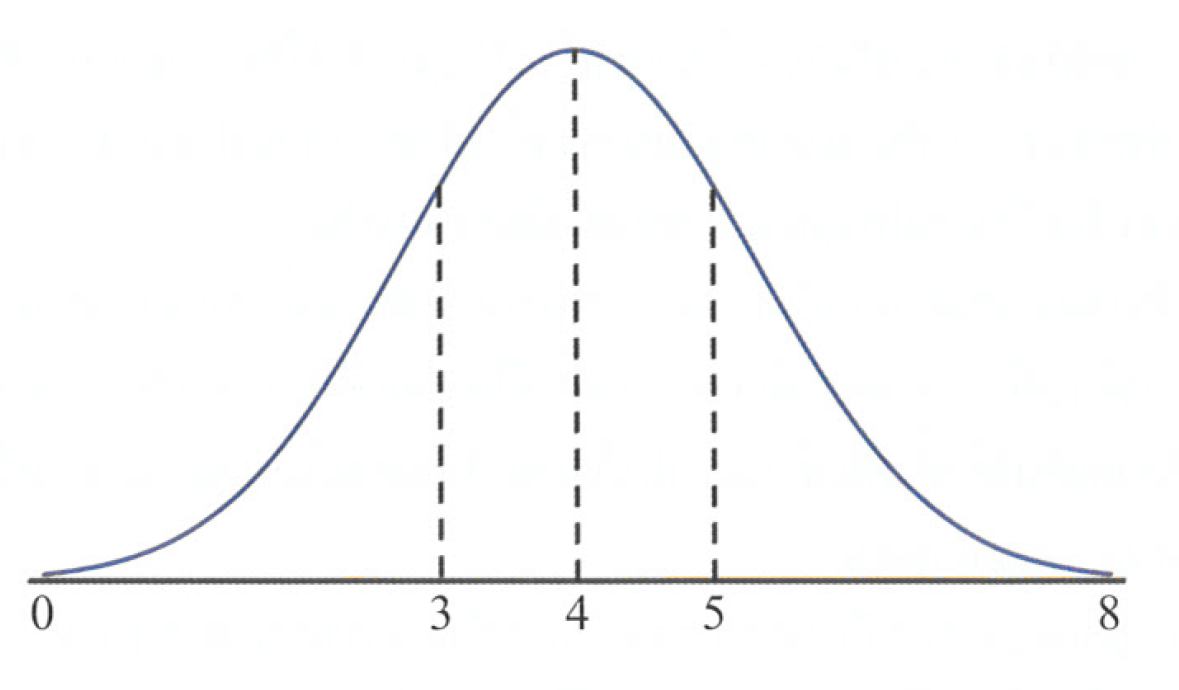
\includegraphics[scale=0.50]{15} 
	\caption{} 
	\label{Figure15} 
\end{figure}
การแจกแจงความน่าจะเป็นของตัวแปรสุ่มที่มีลักษณะเช่นนี้เรียกว่า การแจกแจงปกติ ซึ่งมีบทนิยามดังนี้

\begin{definitionbox}
	\textbf{การแจกแจงปกติ (normal distribution)} คือ การแจกแจงความน่าจะเป็นของตัวแปรสุ่ม ต่อเนื่อง $X$ ที่มีฟังก์ชันความหนาแน่นความน่าจะเป็น คือ
	
	$$
	f(x)=\frac{1}{\sigma \sqrt{2 \pi}} e^{-\frac{1}{2}\left(\frac{x-\mu}{\sigma}\right)^{2}} \text { เมื่อ }-\infty<x<\infty
	$$
	
	โดยที่ $\mu$ แทนค่าเฉลี่ย\\
	และ $\sigma$ แทนส่วนเบี่ยงเบนมาตรฐาน
\end{definitionbox}

การแจกแจงปกติเป็นการแจกแจงความน่าจะเป็นของตัวแปรสุ่มต่อเนื่องที่มีความสำคัญ และใช้มากในสถิติศาสตร์ เนื่องจากเป็นการแจกแจงที่สามารถนำไปใช้วิเคราะห์ข้อมูลในหลายสถานการณ์ เช่น การวิเคราะห์ข้อมูลความสูงของประชากรไทย การวิเคราะห์ข้อมูล อายุการใช้งานของสินค้าที่ผลิตจากโรงงานแห่งหนึ่ง

ถ้าการแจกแจงความน่าจะเป็นของตัวแปรสุ่ม $X$ เป็นการแจกแจงปกติ แล้วเมื่อเขียนกราฟ ของฟังก์ชันความหนาแน่นความน่าจะเป็นสำหรับตัวแปรสุ่ม $X$ จะได้ เส้นโค้งปกติ (normal curve) ซึ่งเป็นเส้นโค้งรูประฆังที่มีสมบัติดังต่อไปนี้

\begin{enumerate}[label=\arabic*., leftmargin=2.5em]
	\item เส้นโค้งมีเส้นตั้งฉากกับแกน $X$ ที่ลากผ่านค่าเฉลี่ยเป็นแกนสมมาตร ทำให้พื้นที่ใต้เส้นโค้ง ทางด้านซ้ายของค่าเฉลี่ยเท่ากับพื้นที่ใต้เส้นโค้งทางด้านขวาของค่าเฉลี่ย
	\item ปลายเส้นโค้งทั้งสองด้านเข้าใกล้แกน $X$ แต่จะไม่ตัดแกน $X$ หรือกล่าวได้ว่าแกน $X$ เป็น เส้นกำกับแนวนอน
	\item ค่าเฉลี่ยและส่วนเบี่ยงเบนมาตรฐาน (หรือความแปรปรวน) จะเป็นตัวกำหนดลักษณะเฉพาะ ของเส้นโค้งว่ามีแกนสมมาตรอยู่ที่ใด และมีการกระจายจากค่าเฉลี่ยมากน้อยเพียงใด
\end{enumerate}

ตัวอย่างเช่น เส้นโค้งปกติที่มีค่าเฉลี่ย $\mu$ และส่วนเบี่ยงเบนมาตรฐาน $\sigma$ สามารถเขียนได้ดังรูป
\begin{figure}[H] 
	\centering 
	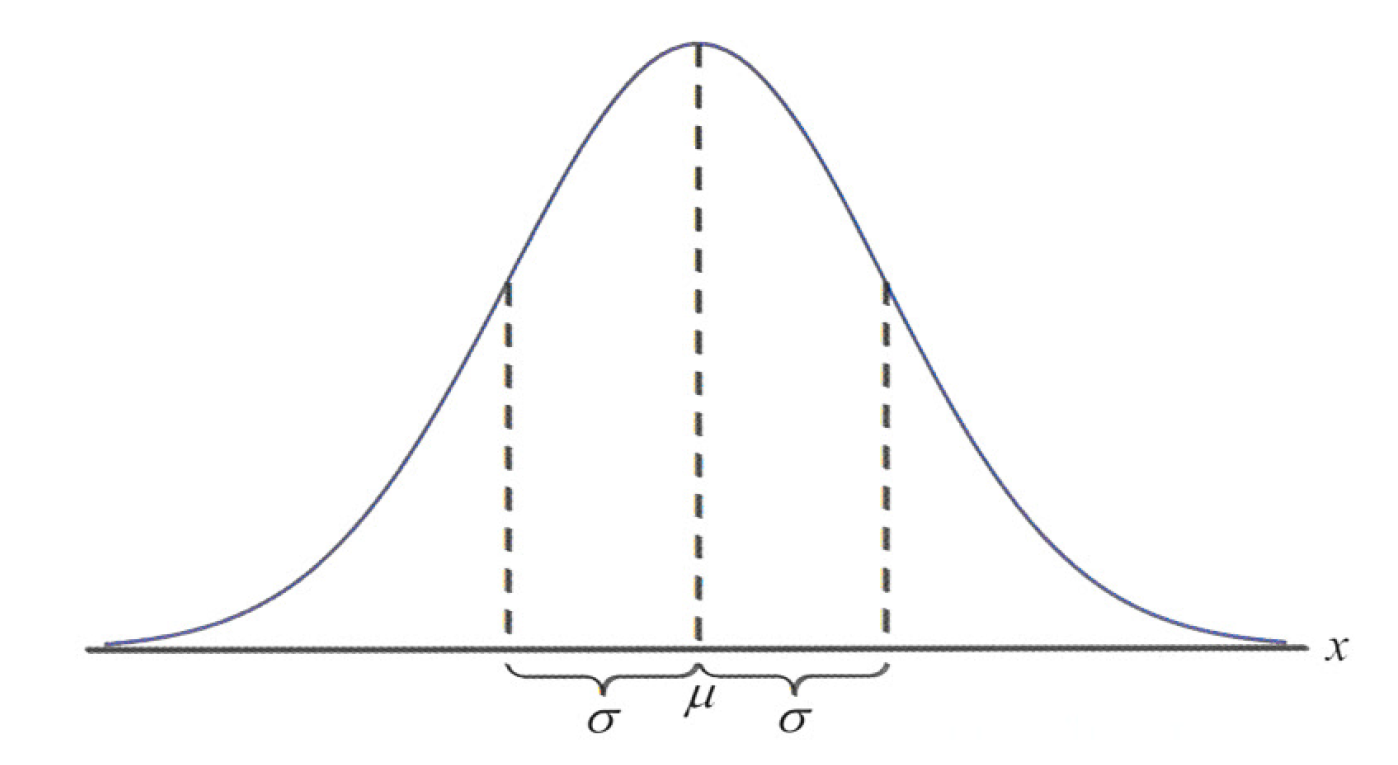
\includegraphics[scale=0.50]{16} 
	\caption{} 
	\label{Figure16} 
\end{figure}

ถ้าค่าเฉลี่ยหรือส่วนเบี่ยงเบนมาตรฐานค่าใดค่าหนึ่งหรือทั้งสองค่าเปลี่ยนแปลงไป เส้นโค้งปกติ จะเปลี่ยนแปลงตามไปด้วย แต่ยังคงเป็นเส้นโค้งรูประฆัง ดังตัวอย่างต่อไปนี้

เมื่อค่าเฉลี่ยแตกต่างกัน แต่ส่วนเบี่ยงเบนมาตรฐานเท่ากัน
\begin{figure}[H] 
	\centering 
	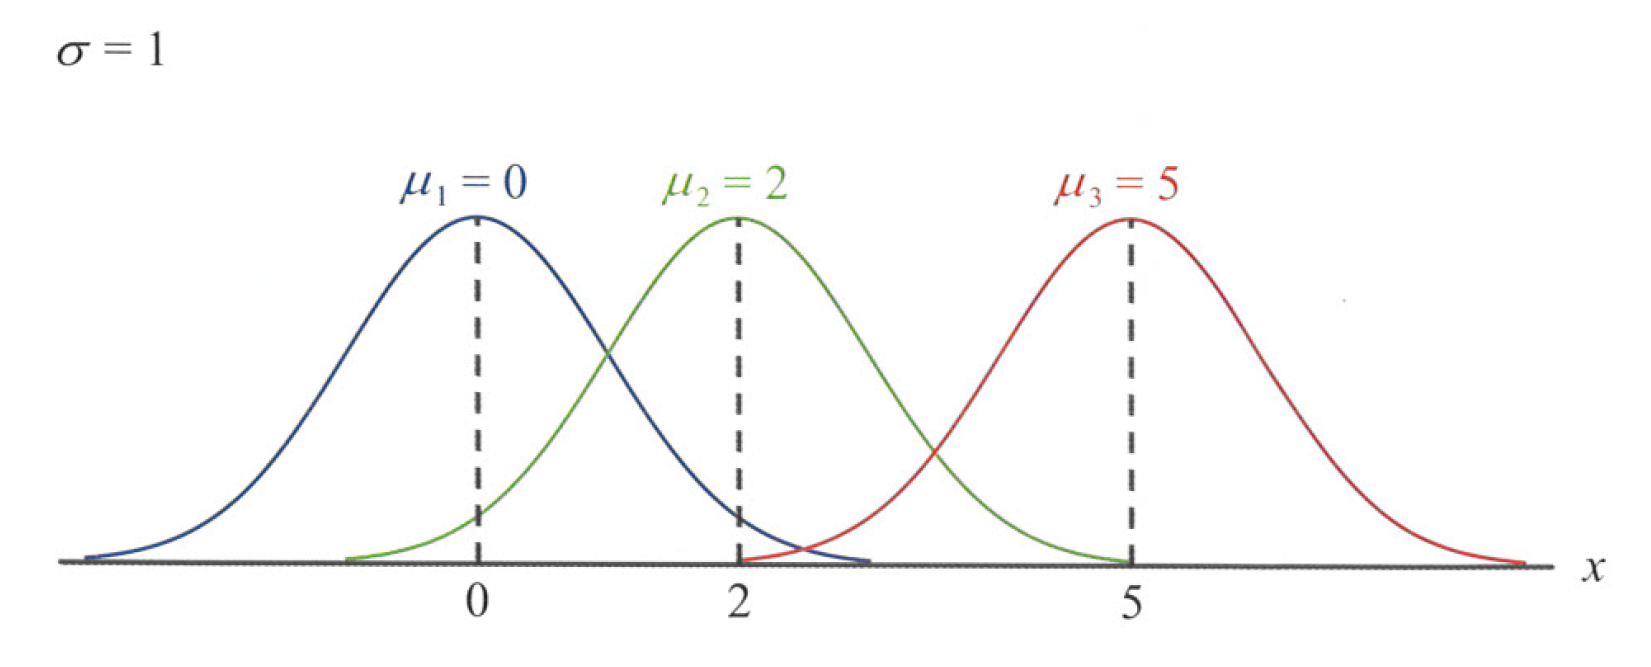
\includegraphics[scale=0.50]{17} 
	\caption{} 
	\label{Figure17} 
\end{figure}

เมื่อส่วนเบี่ยงเบนมาตรฐานแตกต่างกัน แต่ค่าเฉลี่ยเท่ากัน
\begin{figure}[H] 
	\centering 
	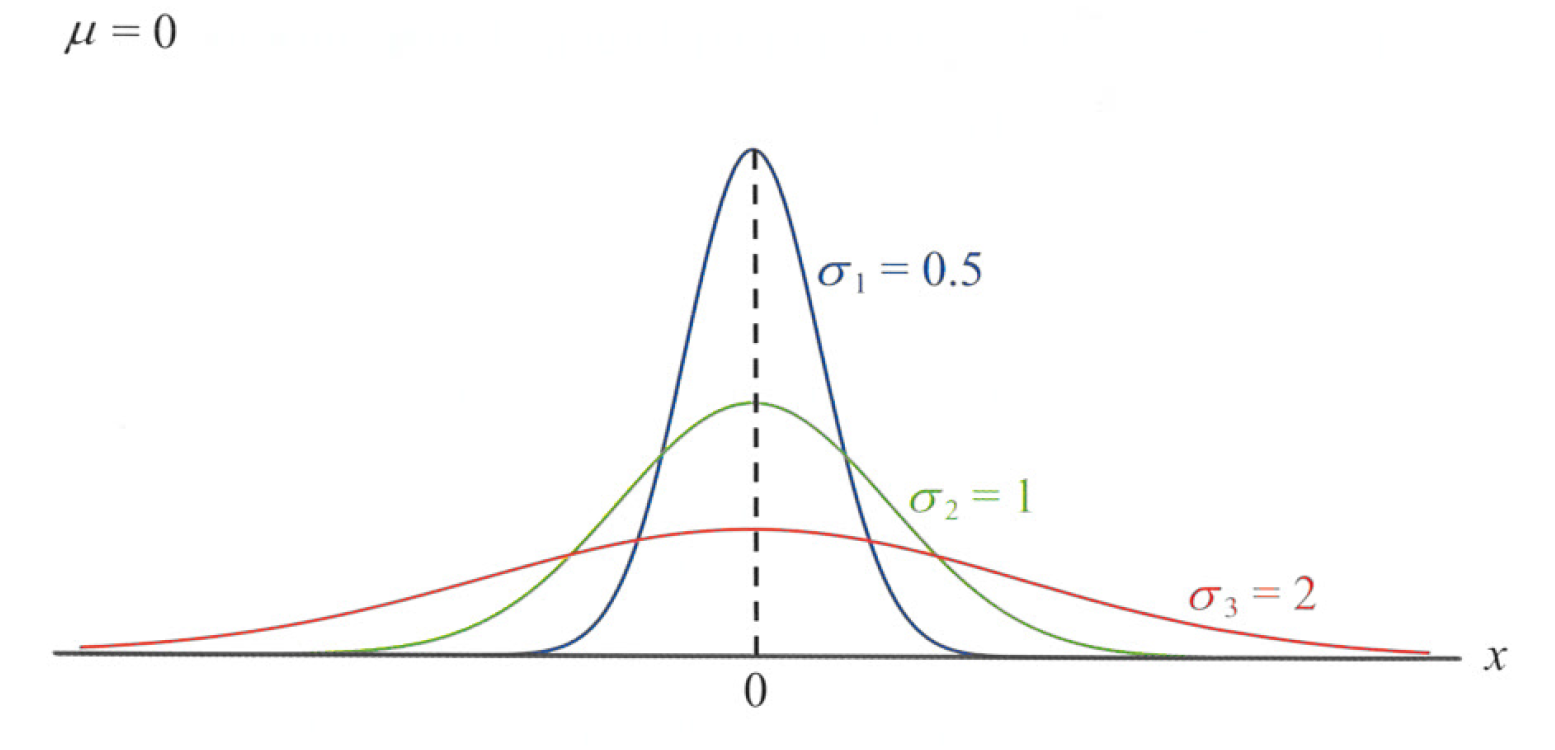
\includegraphics[scale=0.50]{18} 
	\caption{} 
	\label{Figure18} 
\end{figure}

ถ้าตัวแปรสุ่ม $X$ มีการแจกแจงปกติ โดยที่ $\mu$ แทนค่าเฉลี่ย และ $\sigma^{2}$ แทนความแปรปรวน จะเรียกตัวแปรสุ่ม $X$ ว่า \textbf{ตัวแปรสุ่มปกติ} เรียก $\mu$ และ $\sigma^{2}$ ว่า \textbf{พารามิเตอร์ของการแจกแจงปกติ} และเขียนสัญลักษณ์ $X \sim N\left(\mu, \sigma^{2}\right)$ เพื่อแสดงว่าการแจกแจงความน่าจะเป็นของตัวแปรสุ่ม $X$ เป็นการแจกแจงปกติที่มี $\mu$ และ $\sigma^{2}$ เป็นพารามิเตอร์

จากที่กล่าวมาแล้วว่าสามารถหาความน่าจะเป็นที่ตัวแปรสุ่มจะมีค่าอยู่ในช่วงที่สนใจได้จาก การหาพื้นที่ใต้เส้นโค้งความหนาแน่นในช่วงนั้น ซึ่งเท่ากับปริพันธ์จำกัดเขตของฟังก์ชัน ความหนาแน่นความน่าจะเป็นในช่วงดังกล่าว โดยจะต้องใช้วิธีการของแคลคูลัสซึ่งค่อนข้าง ยุ่งยาก ในทางปฏิบัติจึงหาพื้นที่ใต้เส้นโค้งปกติโดยใช้ตารางแสดงพื้นที่ใต้เส้นโค้งปกติ แต่เนื่องจากเป็นไปไม่ได้ที่จะสร้างตารางหลาย ๆ ตารางมาแสดงพื้นที่ใต้เส้นโค้งปกติซึ่งมี ค่าเฉลี่ยและส่วนเบี่ยงเบนมาตรฐานต่างกัน ดังนั้นจะใช้วิธีการแปลงการแจกแจงปกติของ ตัวแปรสุ่มให้เป็นการแจกแจงปกติมาตรฐาน ซึ่งจะกล่าวถึงในหัวข้อต่อไป

\newpage
\section{การแจกแจงปกติมาตรฐาน}
\begin{definitionbox}
	\textbf{การแจกแจงปกติมาตรฐาน (standard normal distribution)} คือ การแจกแจงปกติ ที่มีค่าเฉลี่ยเท่ากับ $0\,(\mu=0)$ และส่วนเบี่ยงเบนมาตรฐานเท่ากับ $1\,(\sigma=1)$
\end{definitionbox}

จะได้ว่าฟังก์ชันความหนาแน่นความน่าจะเป็นของตัวแปรสุ่ม $Z$ ที่มีการแจกแจงปกติมาตรฐาน คือ

$$
f(z)=\frac{1}{\sqrt{2 \pi}} e^{-\frac{z^{2}}{2}} \text { เมื่อ }-\infty<z<\infty
$$

เรียกเส้นโค้งปกติซึ่งได้จากตัวแปรสุ่มปกติที่มีค่าเฉลี่ยเป็น $0$ และส่วนเบี่ยงเบนมาตรฐาน เป็น $1$ ว่า \textbf{เส้นโค้งปกติมาตรฐาน (standard normal curve)} ดังรูป
\begin{figure}[H] 
	\centering 
	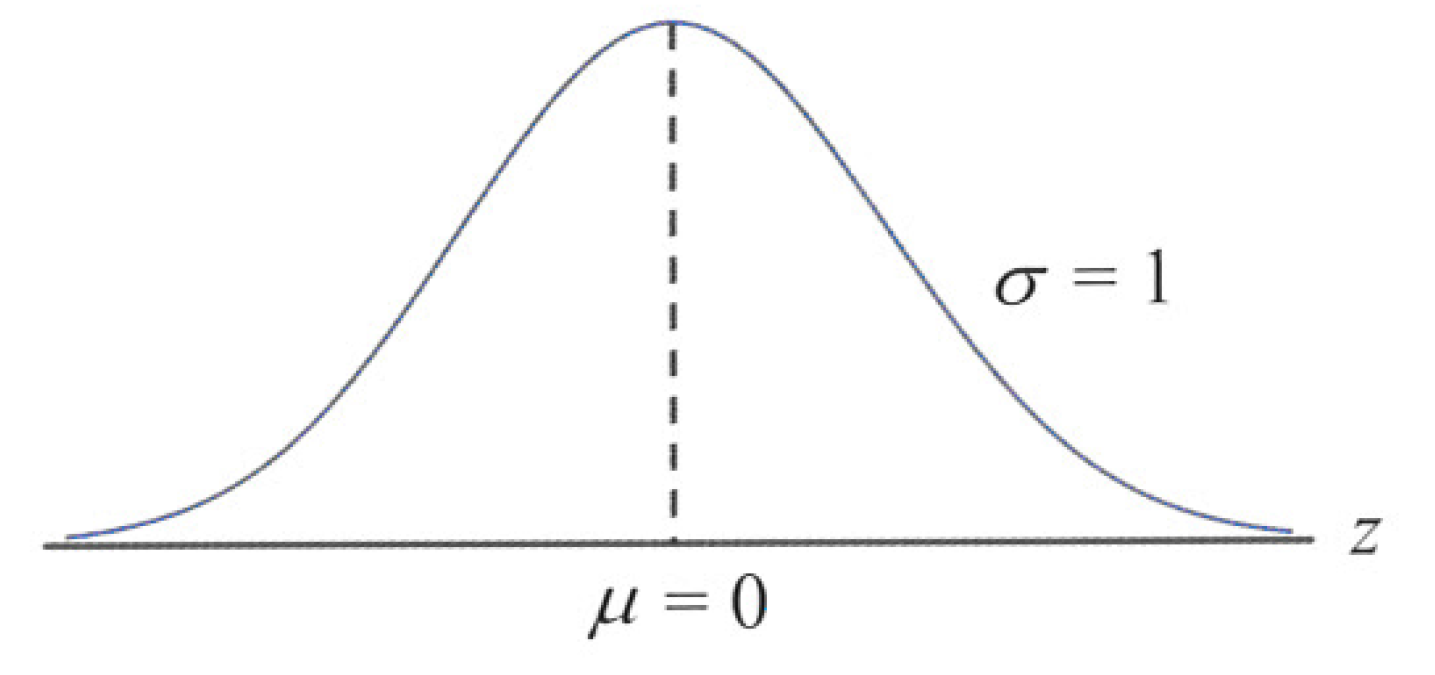
\includegraphics[scale=0.50]{19} 
	\caption{} 
	\label{Figure19} 
\end{figure}

เรียกตัวแปรสุ่มที่มีการแจกแจงปกติมาตรฐานว่า \textbf{ตัวแปรสุ่มปกติมาตรฐาน (standard normal random variable)}

สำหรับการหาความน่าจะเป็นที่ตัวแปรสุ่มปกติมาตรฐานจะมีค่าอยู่ในช่วงที่สนใจ จะใช้ ตารางแสดงพื้นที่ใต้เส้นโค้งปกติมาตรฐาน (ตารางที่ $1$) แทนการหาปริพันธ์จำกัดเขตของ ฟังก์ชันความหนาแน่นความน่าจะเป็น โดยค่าที่ปรากฏในตารางที่ $1$ คือค่าประมาณของพื้นที่ ใต้เส้นโค้งปกติมาตรฐานจาก $-\infty$ ถึง $z$ หรือความน่าจะเป็นที่ตัวแปรสุ่มปกติมาตรฐาน $Z$ มีค่าน้อยกว่าหรือเท่ากับ $z$ เขียนแทนด้วยสัญลักษณ์ $P(Z \leq z)$

การอ่านตารางที่ $1$ ให้เริ่มพิจารณาจากแถวที่แสดงค่า $z$ จาก $0.0$ ถึง $-3.0$ หรือจาก $0.0$ ถึง $3.0$ ค่าของ $z$ มีค่าลดลงหรือเพิ่มขึ้นแถวละ $0.1$ จากนั้นจึงพิจารณาหลักซึ่งแสดงทศนิยม ตำแหน่งที่ $2$ ของค่า $z$ เช่น ถ้าต้องการหา $P(Z \leq -1.54)$ จะเริ่มพิจารณาจากแถวที่แสดง ค่า $z = -1.5$ จากนั้นพิจารณาหลักที่แสดงค่า $0.04$ จะได้ว่าพื้นที่ใต้เส้นโค้งปกติมาตรฐาน จาก $-\infty$ ถึง $-1.54$ หรือ $P(Z \leq -1.54)$ มีค่าประมาณ $0.0618$

\newpage
\begin{examplebox}
ให้ $Z$ เป็นตัวแปรสุ่มปกติมาตรฐาน จงหา
\begin{enumerate}[label=\arabic*), leftmargin=*]
	\item $P(Z \leq 2)$
	\item $P(Z>1.29)$
	\item $P(-1.27 \leq Z \leq 0.45)$
\end{enumerate}
\end{examplebox}
\solution
\newpage

ในกรณีที่ตัวแปรสุ่มมีการแจกแจงปกติแต่ไม่ใช่การแจกแจงปกติมาตรฐาน จะไม่สามารถใช้ ตารางที่ $1$ ในการหาความน่าจะเป็นได้ ดังนั้นจะต้องแปลงตัวแปรสุ่มปกติให้เป็นตัวแปรสุ่ม ปกติมาตรฐาน โดยใช้ทฤษฎีบทต่อไปนี้
\begin{theorembox}
ให้ตัวแปรสุ่ม $X$ มีการแจกแจงปกติ โดยมีค่าเฉลี่ย $\mu$ และส่วนเบี่ยงเบนมาตรฐาน $\sigma$ ถ้าตัวแปรสุ่ม $Z$ นิยามโดย $Z=\dfrac{X-\mu}{\sigma}$ แล้ว ตัวแปรสุ่ม $Z$ จะมีการแจกแจงปกติ มาตรฐาน นั่นคือ $\mu_{Z}=0$ และ $\sigma_{Z}=1$

นอกจากนี้ $P(a \leq X \leq b)=P\left(\dfrac{a-\mu}{\sigma} \leq Z \leq \dfrac{b-\mu}{\sigma}\right)$ เมื่อ $a, b$ เป็นค่าที่เป็นไปได้ของ ตัวแปรสุ่ม $X$ และ $a \leq b$
\end{theorembox}

\begin{examplebox}
กำหนดให้ $X \sim N(3.5,4)$ จงหา $P(2.4<X<5.2)$
\end{examplebox}
\solution
\newpage

สำหรับตัวแปรสุ่มปกติ $X$ ที่มีค่าเฉลี่ย $\mu$ และส่วนเบี่ยงเบนมาตรฐาน $\sigma$ และ ตัวแปรสุ่ม $Z$ นิยามโดย 
\[Z=\dfrac{X-\mu}{\sigma}\]
จะได้ว่า

1. $P(\mu-\sigma \leq X \leq \mu+\sigma)=P(-1 \leq Z \leq 1)$
$$
\begin{aligned}
	& =P(Z \leq 1)-P(Z<-1) \\
	& =0.8413-0.1587 \\
	& =0.6826
\end{aligned}
$$
\begin{figure}[H] 
	\centering 
	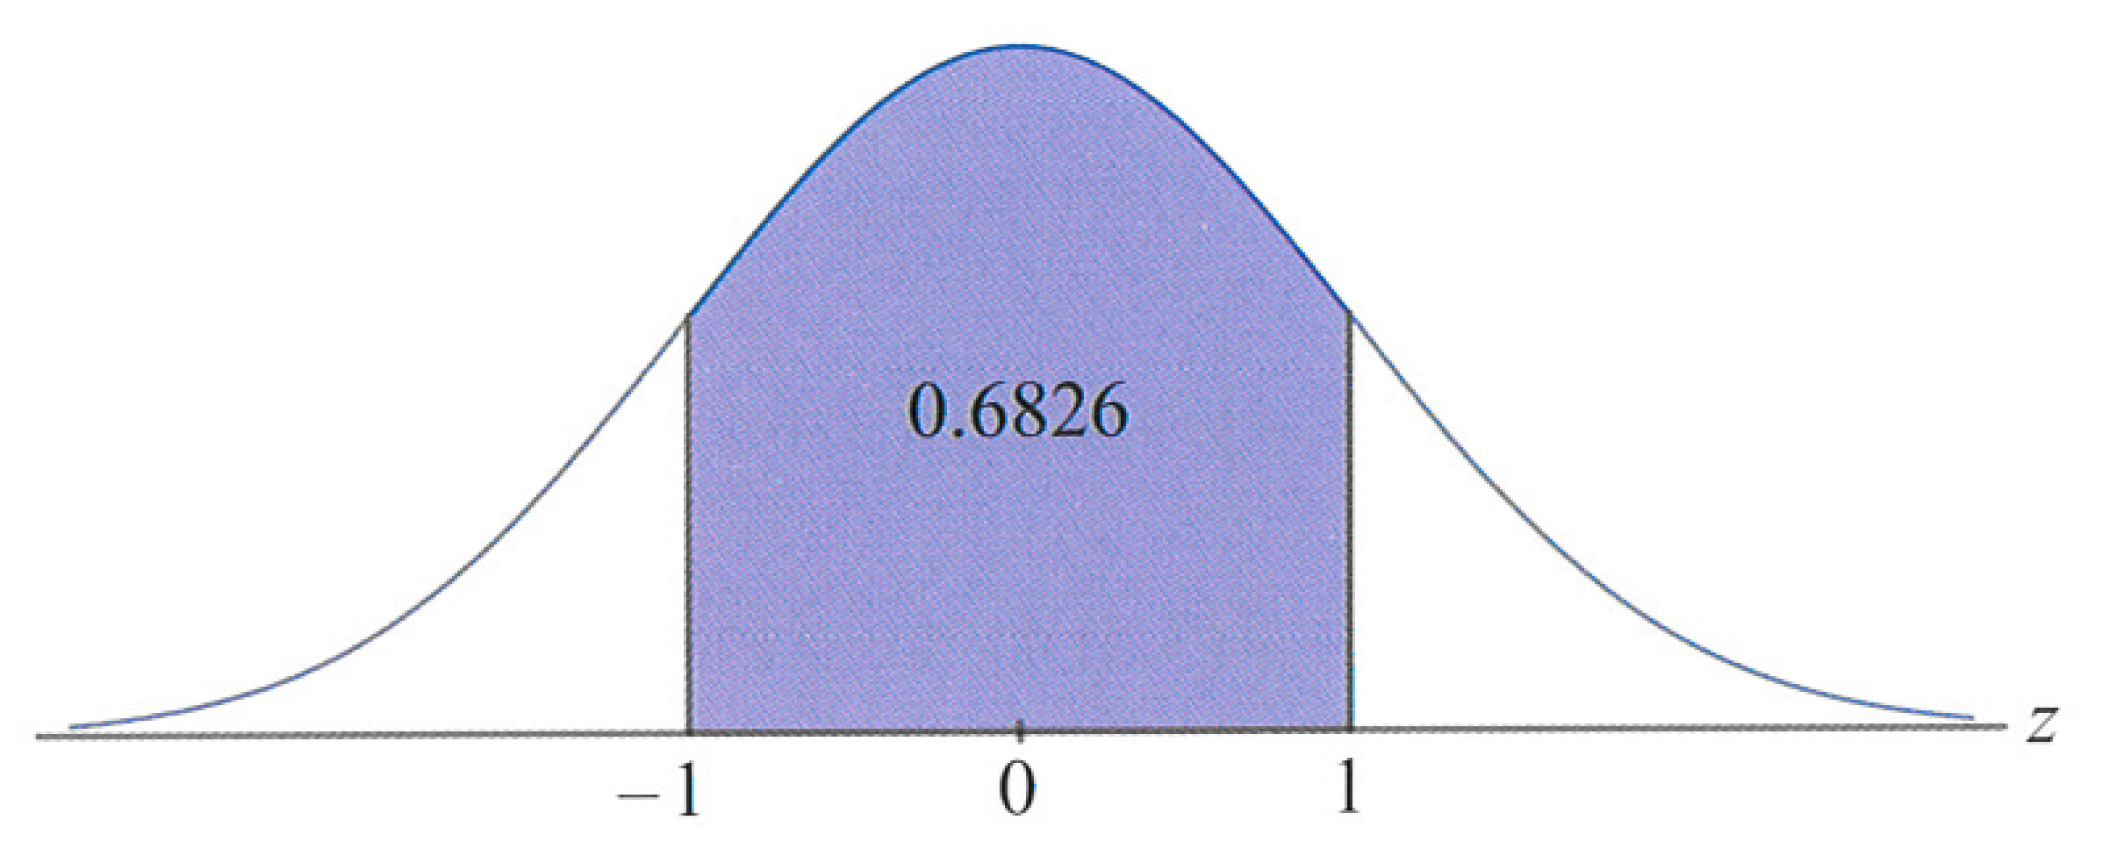
\includegraphics[scale=0.40]{20} 
	\caption{} 
	\label{Figure20} 
\end{figure}
นั่นคือ ความน่าจะเป็นที่ตัวแปรสุ่ม $X$ จะมีค่าอยู่ในช่วง $[\mu-\sigma, \mu+\sigma]$ มีค่าประมาณ $0.6826$ หรือพื้นที่ใต้เส้นโค้งปกติจาก $\mu-\sigma$ ถึง $\mu+\sigma$ มีค่าประมาณ $68.26\%$ ของพื้นที่ใต้เส้นโค้งปกติทั้งหมด
\begin{figure}[H] 
	\centering 
	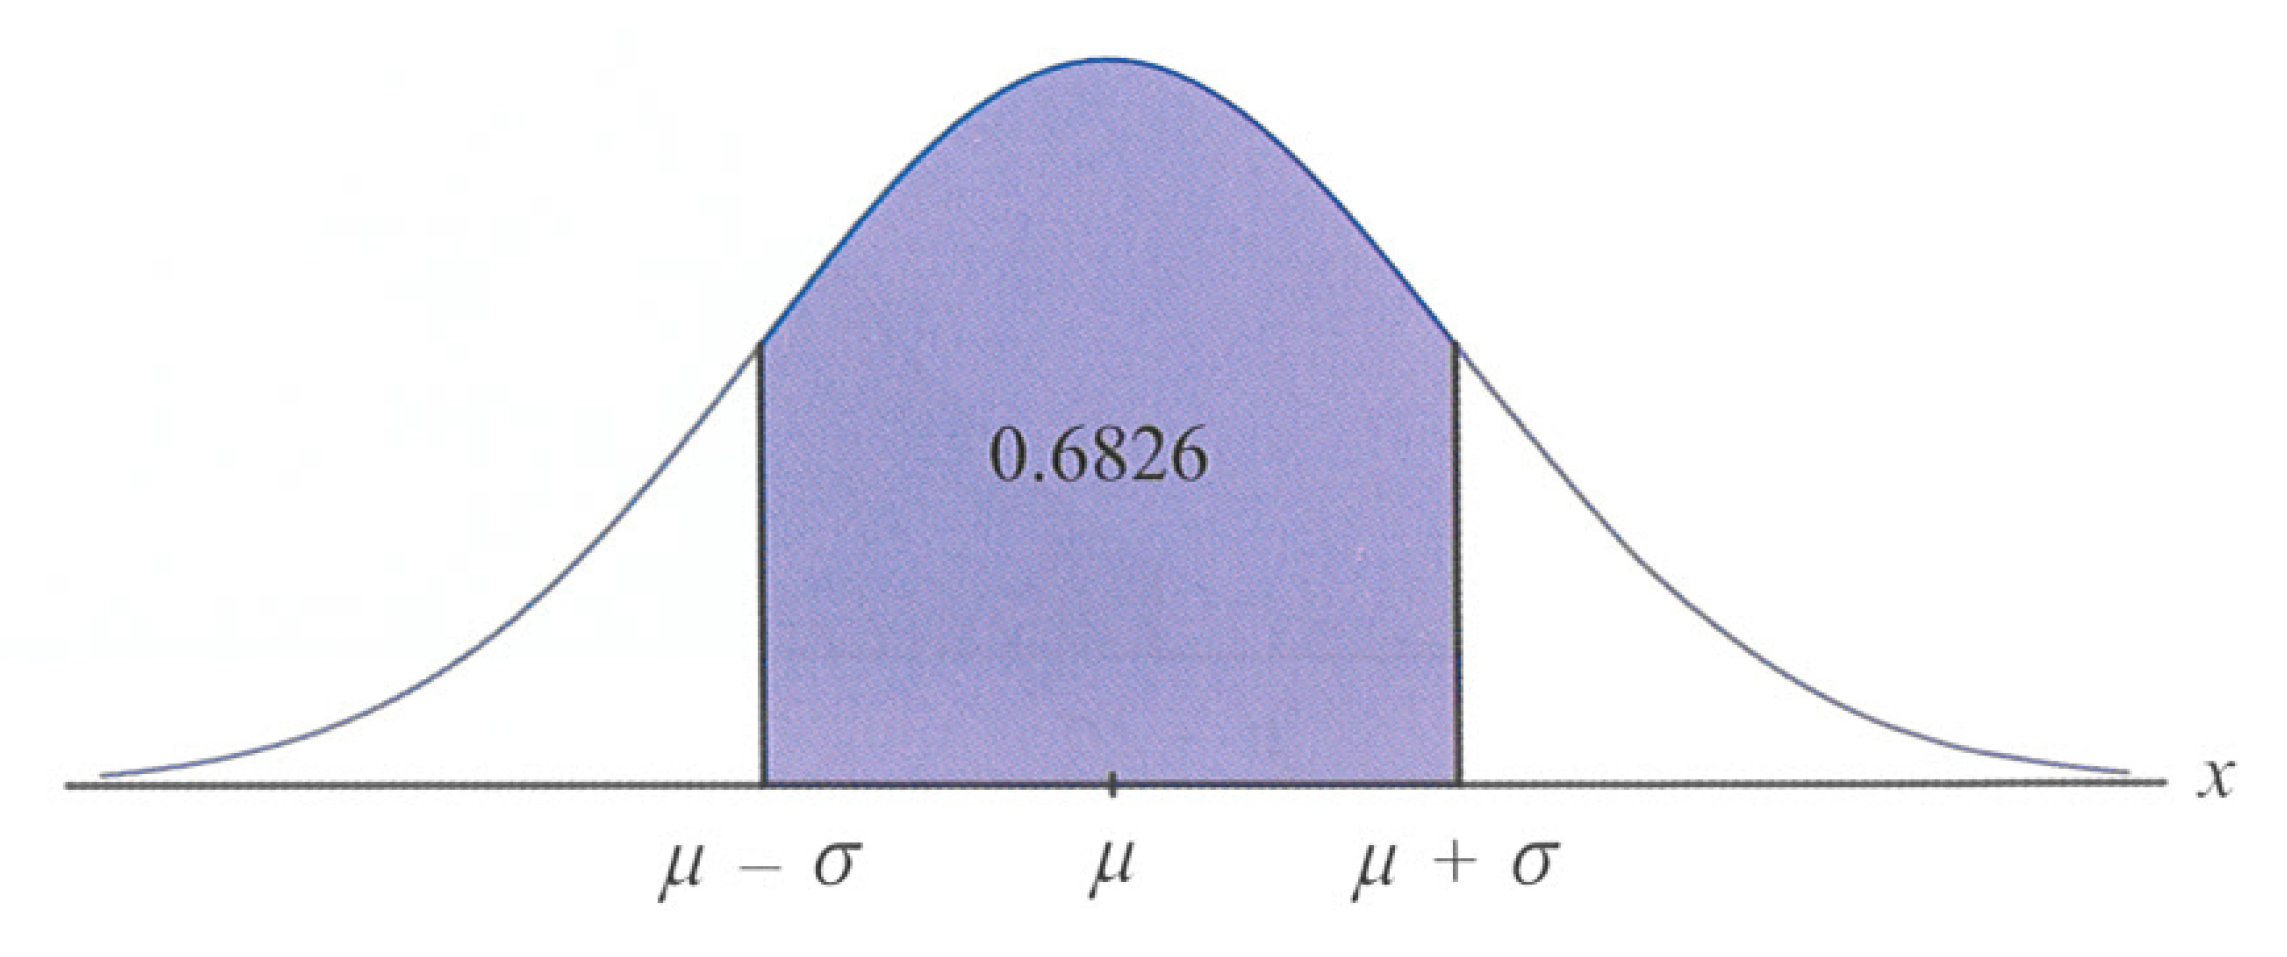
\includegraphics[scale=0.40]{21} 
	\caption{} 
	\label{Figure21} 
\end{figure}

\newpage
2. $P(\mu-2\sigma \leq X \leq \mu+2\sigma)=P(-2 \leq Z \leq 2)$
$$
\begin{aligned}
	& =P(Z \leq 2)-P(Z<-2) \\
	& =0.9772-0.0228 \\
	& =0.9544
\end{aligned}
$$
\begin{figure}[H] 
	\centering 
	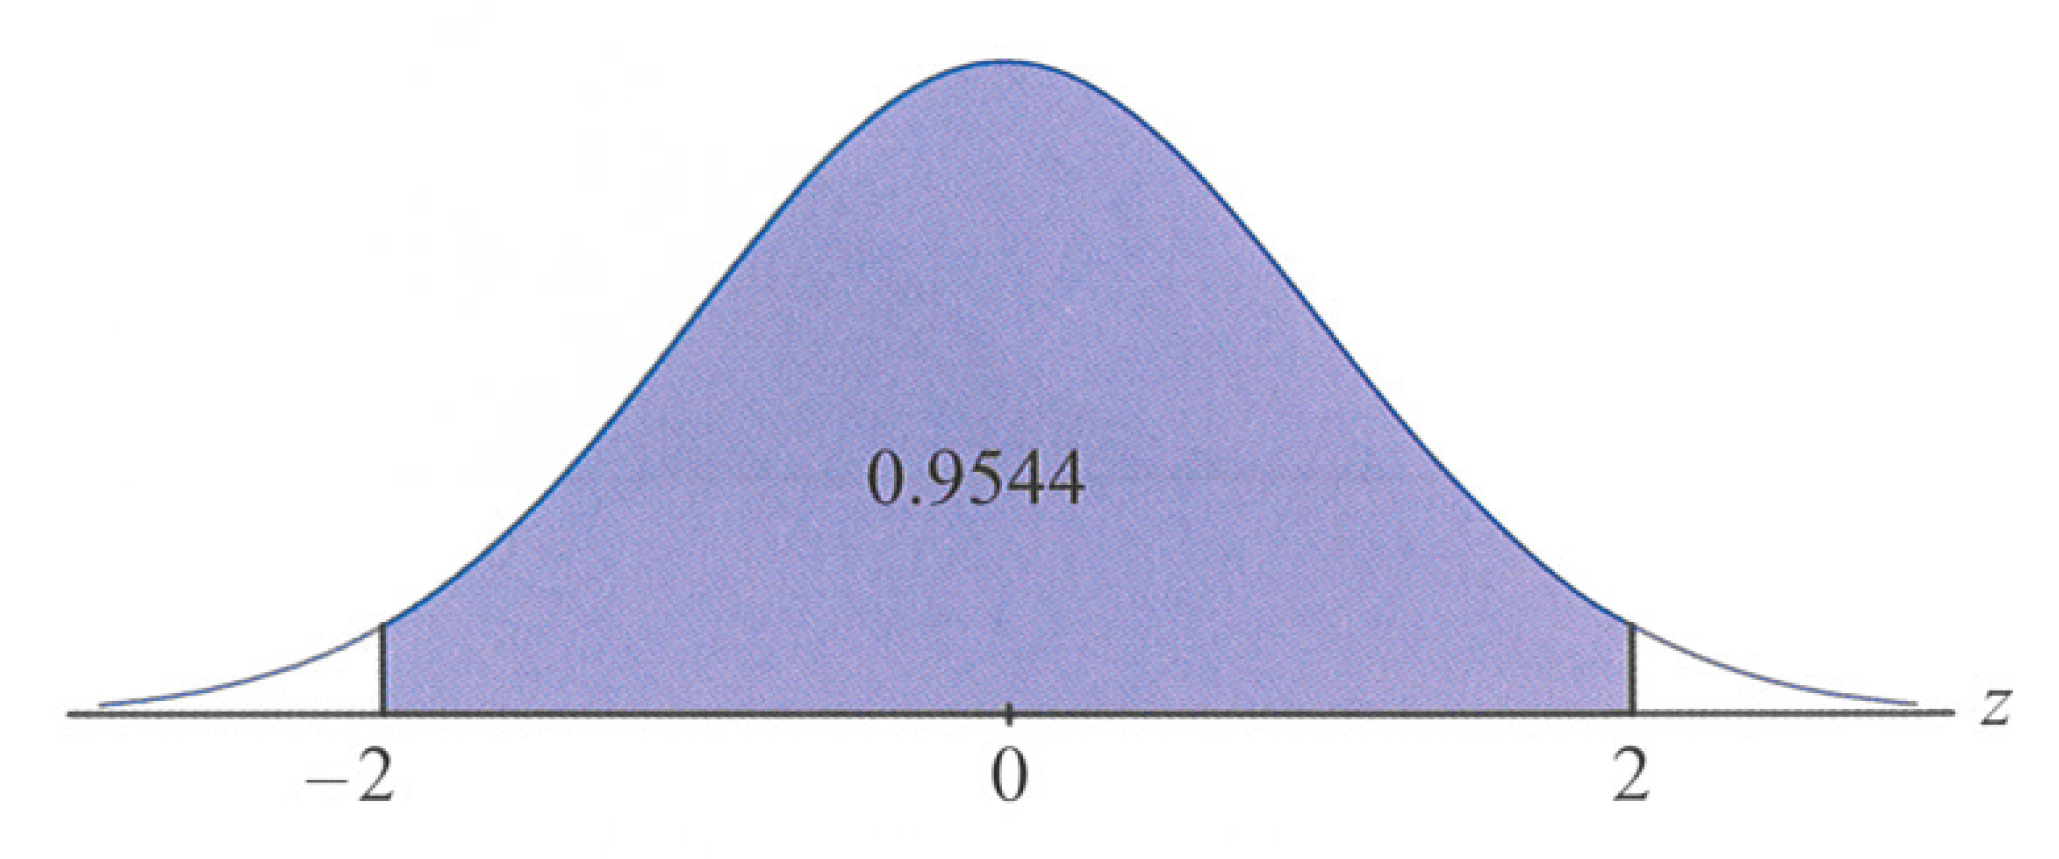
\includegraphics[scale=0.40]{22} 
	\caption{} 
	\label{Figure22} 
\end{figure}
นั่นคือ ความน่าจะเป็นที่ตัวแปรสุ่ม $X$ จะมีค่าอยู่ในช่วง $[\mu-2\sigma, \mu+2\sigma]$ มีค่า ประมาณ $0.9544$ หรือพื้นที่ใต้เส้นโค้งปกติจาก $\mu-2\sigma$ ถึง $\mu+2\sigma$ มีค่าประมาณ $95.44\%$ ของพื้นที่ใต้เส้นโค้งปกติทั้งหมด
\begin{figure}[H] 
	\centering 
	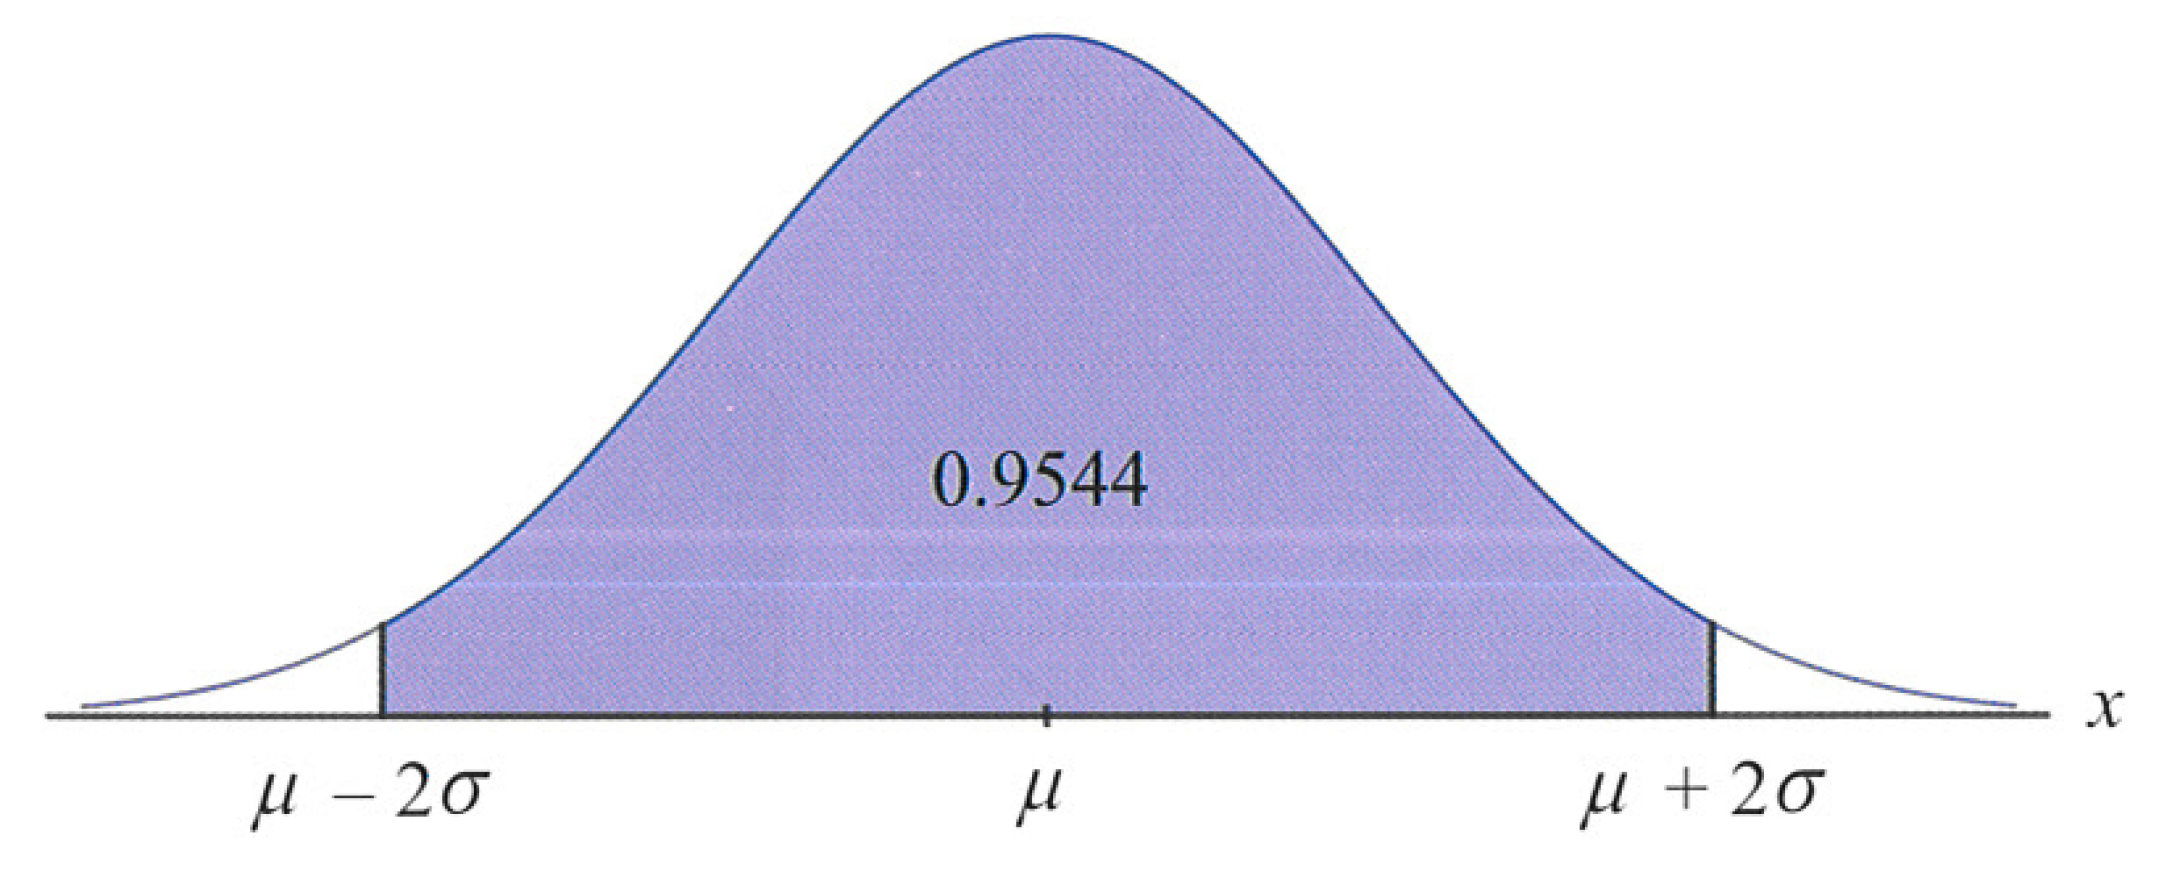
\includegraphics[scale=0.40]{23} 
	\caption{} 
	\label{Figure23} 
\end{figure}

3. $P(\mu-3\sigma \leq X \leq \mu+3\sigma)=P(-3 \leq Z \leq 3)$

$$
\begin{aligned}
	& =P(Z \leq 3)-P(Z<-3) \\
	& =0.9987-0.0013 \\
	& =0.9974
\end{aligned}
$$
\begin{figure}[H] 
	\centering 
	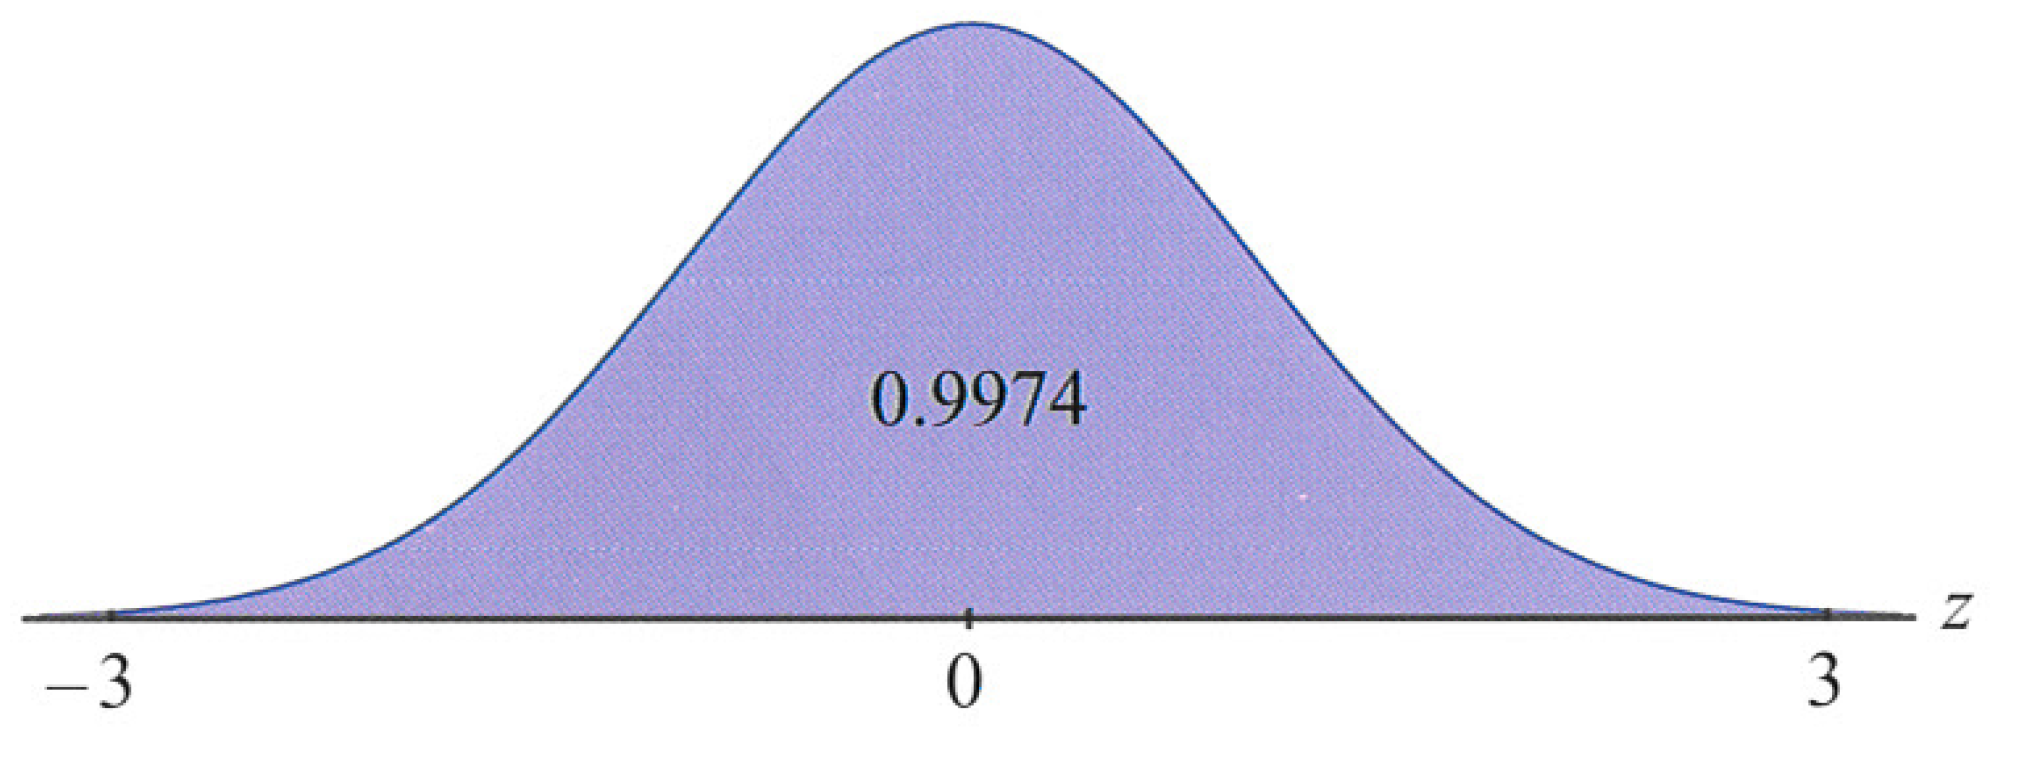
\includegraphics[scale=0.40]{24} 
	\caption{} 
	\label{Figure24} 
\end{figure}

นั่นคือ ความน่าจะเป็นที่ตัวแปรสุ่ม $X$ จะมีค่าอยู่ในช่วง $[\mu-3\sigma, \mu+3\sigma]$ มีค่า ประมาณ $0.9974$ หรือพื้นที่ใต้เส้นโค้งปกติจาก $\mu-3\sigma$ ถึง $\mu+3\sigma$ มีค่าประมาณ $99.74\%$ ของพื้นที่ใต้เส้นโค้งปกติทั้งหมด
\begin{figure}[H] 
	\centering 
	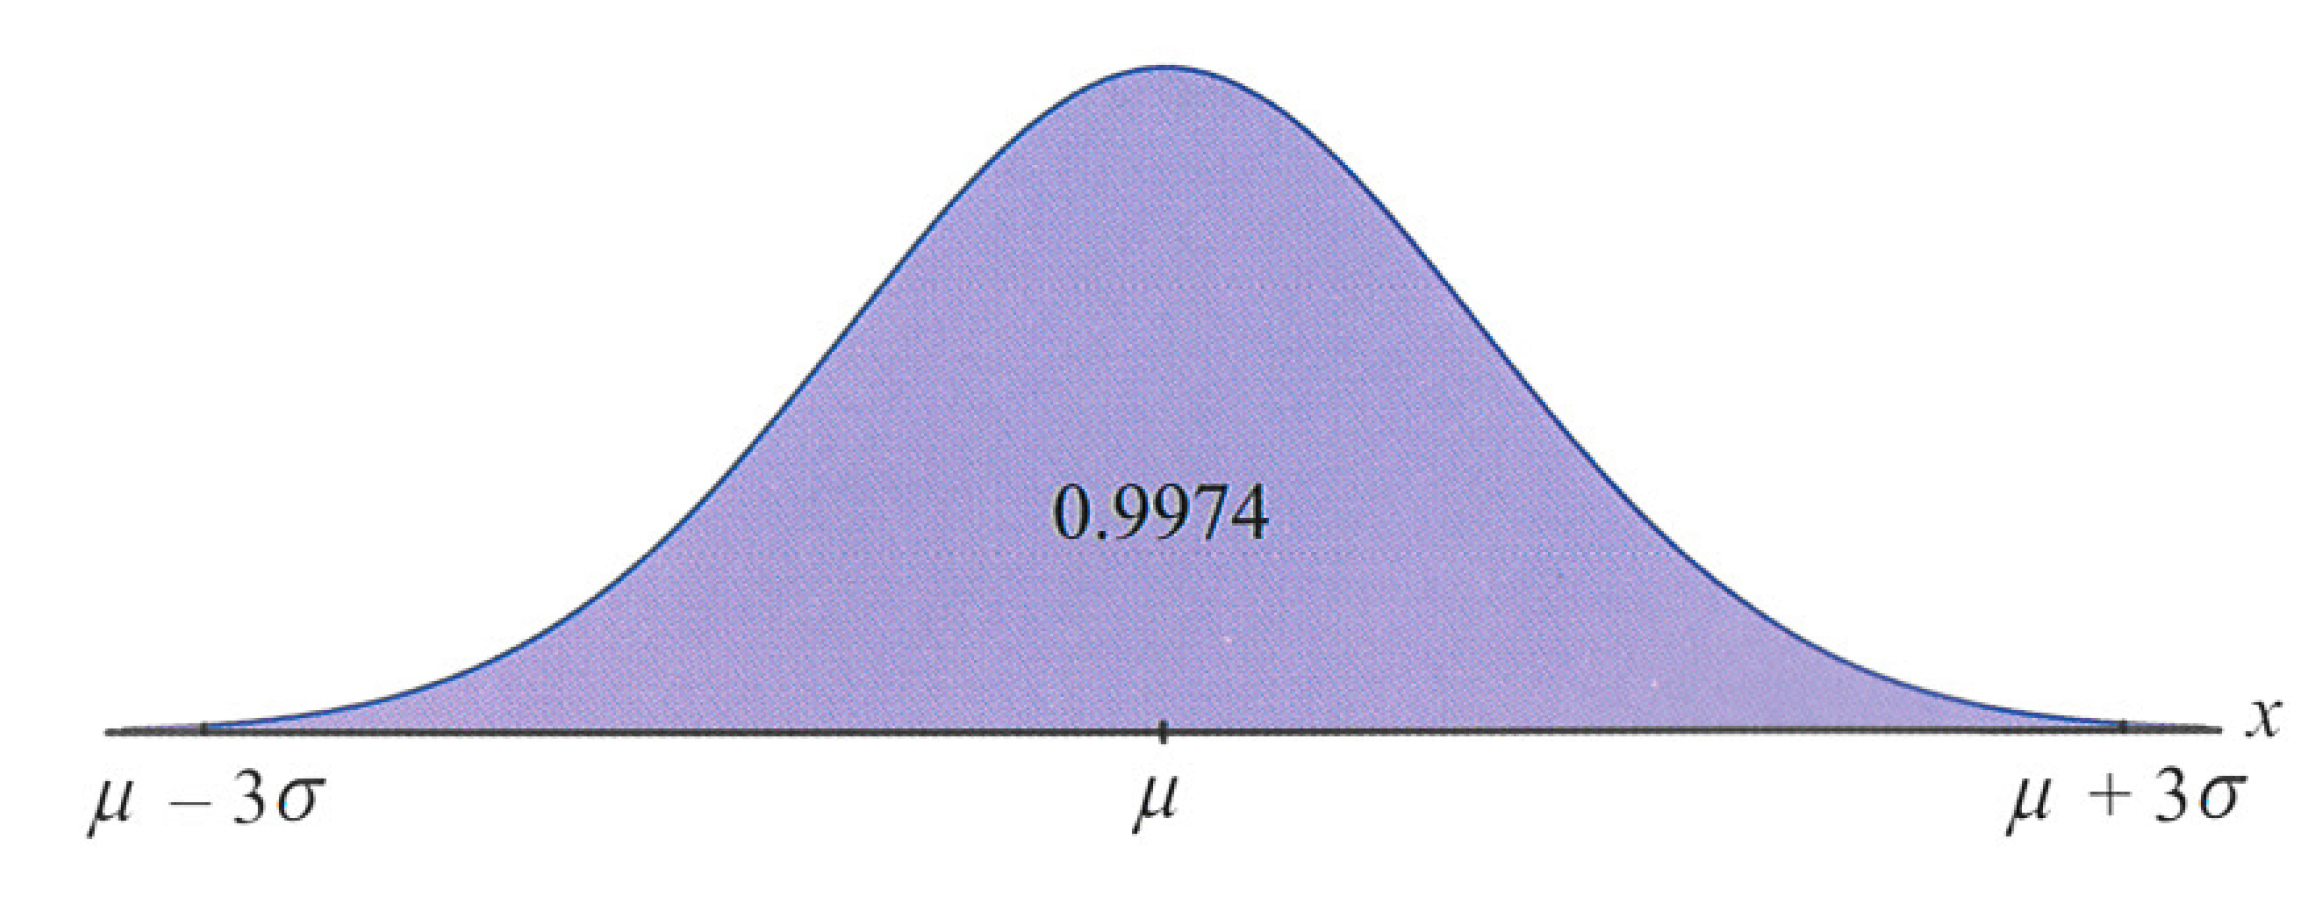
\includegraphics[scale=0.40]{25} 
	\caption{} 
	\label{Figure25} 
\end{figure}
\newpage
\begin{examplebox}
ความสูงของนักเรียนชั้นมัธยมศึกษาปีที่ $6$ ของโรงเรียนแห่งหนึ่งมีการแจกแจงปกติ โดยมี ค่าเฉลี่ยและส่วนเบี่ยงเบนมาตรฐานเท่ากับ $160$ และ $5$ เซนติเมตร ตามลำดับ ถ้าสุ่มนักเรียน ชั้นมัธยมศึกษาปีที่ $6$ จำนวน $1$ คนจากโรงเรียนนี้ จงหาความน่าจะเป็นที่นักเรียนที่สุ่มได้ จะมีความสูง
\begin{enumerate}[label=\arabic*), leftmargin=*]
	\item ระหว่าง $150$ และ $170$ เซนติเมตร
	\item มากกว่า $162$ เซนติเมตร
\end{enumerate}
\end{examplebox}
\solution ให้ตัวแปรสุ่ม $X$ คือความสูงของนักเรียนชั้นมัธยมศึกษาปีที่ $6$ ของโรงเรียนแห่งนี้ จะได้ว่าตัวแปรสุ่ม $X$ มีการแจกแจงปกติ โดยที่ $\mu = 160$ และ $\sigma = 5$

เมื่อแปลงตัวแปรสุ่ม $X$ ให้เป็นตัวแปรสุ่มปกติมาตรฐาน $Z$ จะได้
\begin{equation*}
	Z = \frac{X - \mu}{\sigma}
\end{equation*}
\newpage
\subsection{เปอร์เซ็นไทล์ของตัวแปรสุ่มต่อเนื่อง}
จากหัวข้อ $3.3$ นักเรียนทราบแล้วว่าเปอร์เซ็นไทล์เป็นค่าวัดตำแหน่งที่ของข้อมูลเชิงปริมาณ โดยแบ่งข้อมูลที่เรียงจากน้อยไปมากออกเป็น $100$ ส่วน เท่า ๆ กัน สำหรับตัวแปรสุ่มต่อเนื่อง $X$ เนื่องจากพื้นที่ใต้เส้นโค้งความหนาแน่นทั้งหมดเท่ากับ $1$ หรือคิดเป็น $100\%$ ดังนั้น ถ้า $x$ เป็น ค่าที่เป็นไปได้ของตัวแปรสุ่ม $X$ จะได้ว่าข้อมูลที่มีค่าน้อยกว่า $x$ มีจำนวน $P(X<x) \cdot 100\%$ นั่นคือ ถ้า $P(X<x) \cdot 100$ เป็นจำนวนเต็มที่อยู่ระหว่าง $0$ และ $100$ จะได้ว่าเปอร์เซ็นไทล์ ที่ $P(X<x) \cdot 100$ เท่ากับ $x$

ตัวอย่างเช่น ถ้า $Z$ เป็นตัวแปรสุ่มปกติมาตรฐาน เนื่องจาก $P(Z<0)=0.5$ ดังนั้น $0$ คือเปอร์เซ็นไทล์ที่ $P(Z<0) \cdot 100=(0.5)(100)=50$ หรือกล่าวได้ว่าข้อมูลที่มีค่าน้อยกว่า $0$ มีจำนวน $50\%$ ของข้อมูลทั้งหมด โดยเมื่อพิจารณาจากรูปต่อไปนี้จะเห็นว่าบริเวณที่แรเงา มีพื้นที่เป็นครึ่งหนึ่งของพื้นที่ใต้เส้นโค้งปกติมาตรฐานทั้งหมด
\begin{figure}[H] 
	\centering 
	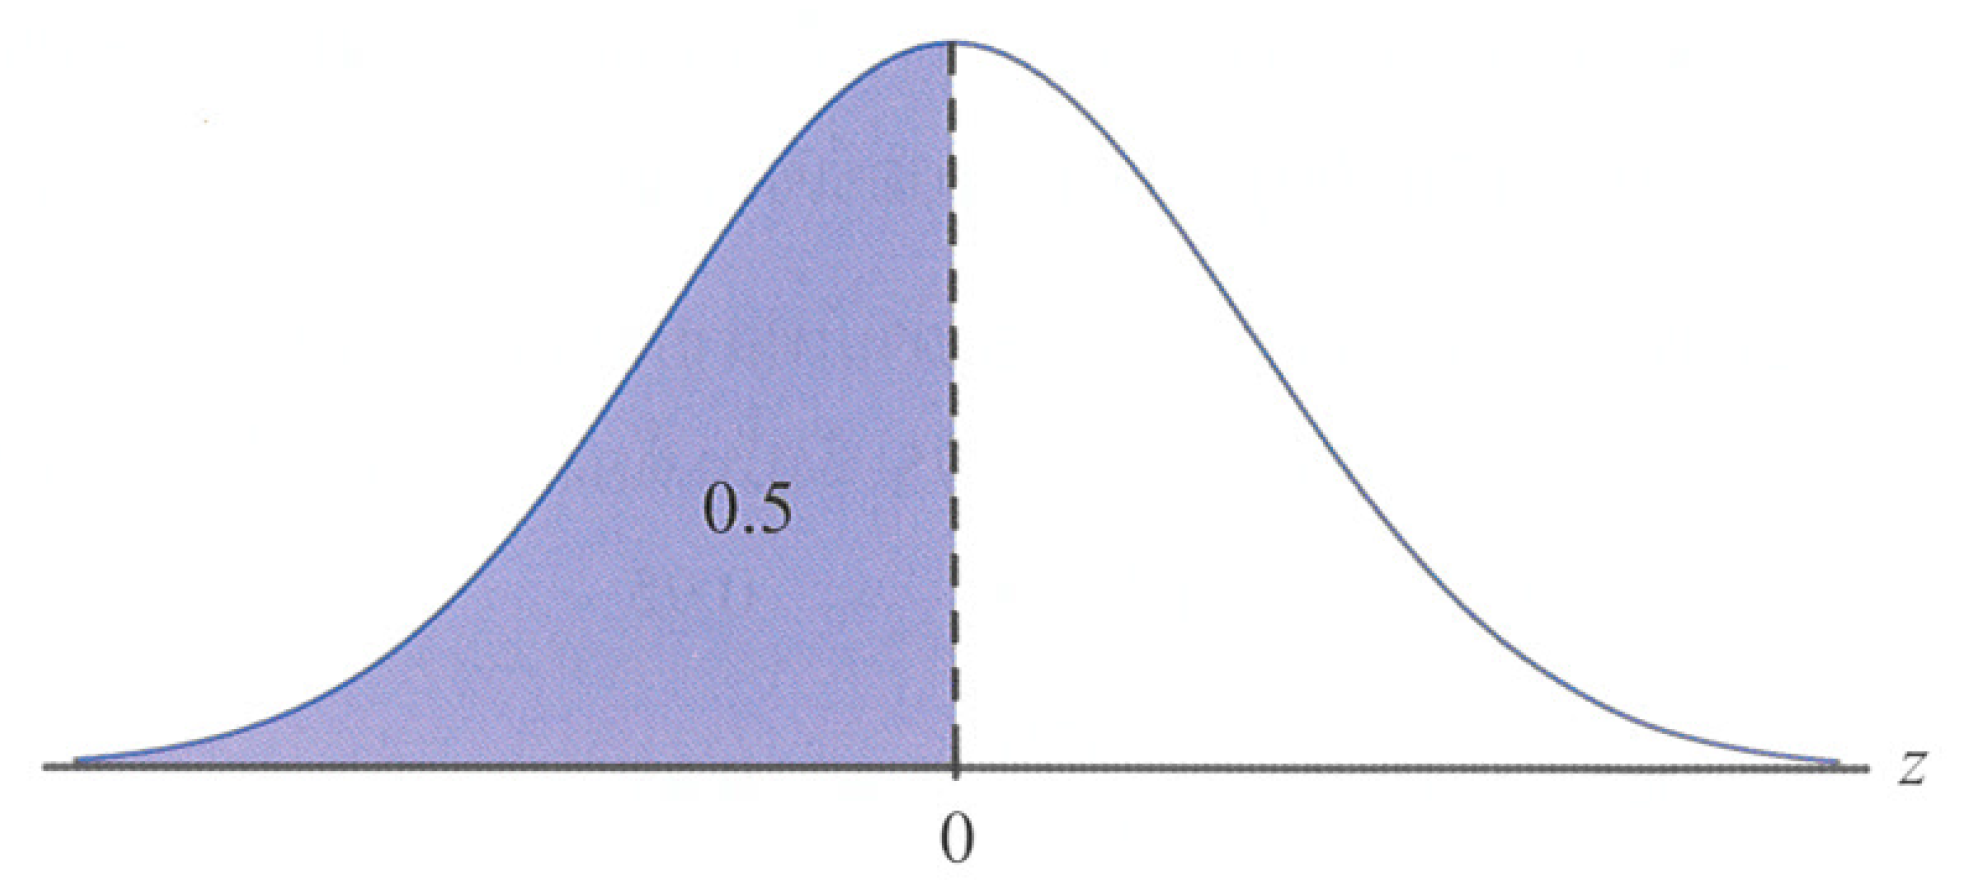
\includegraphics[scale=0.40]{26} 
	\caption{} 
	\label{Figure26} 
\end{figure}
\newpage
\begin{examplebox}
อายุการใช้งานของถ่านไฟฉายชนิดหนึ่งมีการแจกแจงปกติ โดยค่าเฉลี่ยและส่วนเบี่ยงเบน มาตรฐานเท่ากับ $756$ และ $35$ นาที ตามลำดับ จงหาว่า
	\begin{enumerate}[label=\arabic*), leftmargin=*]
\item ถ่านไฟฉายที่มีอายุการใช้งานน้อยกว่า $791$ นาที มีกี่เปอร์เซ็นต์ของถ่านไฟฉายทั้งหมด
\item ถ่านไฟฉายที่มีอายุการใช้งานมากกว่าหรือเท่ากับเปอร์เซ็นไทล์ที่ $95$ สามารถใช้งานได้อย่างน้อย กี่นาที เมื่อกำหนดให้ $P(Z<1.645)=0.95$
	\end{enumerate}
\end{examplebox}
\solution ให้ตัวแปรสุ่ม $X$ คืออายุการใช้งานของถ่านไฟฉาย จะได้ว่าตัวแปรสุ่ม $X$ มีการแจกแจงปกติ โดยที่ $\mu = 756$ และ $\sigma = 35$

เมื่อแปลงตัวแปรสุ่ม $X$ ให้เป็นตัวแปรสุ่มปกติมาตรฐาน $Z$ จะได้
\begin{equation*}
	Z = \frac{X - \mu}{\sigma}
\end{equation*}
\newpage
\subsection{การเปรียบเทียบตำแหน่งของข้อมูลโดยใช้ค่าของตัวแปรสุ่มปกติมาตรฐาน}
การแปลงตัวแปรสุ่มปกติให้เป็นตัวแปรสุ่มปกติมาตรฐาน นอกจากจะมีประโยชน์ในการหา ความน่าจะเป็นโดยใช้ตารางแล้ว ยังสามารถนำค่าของตัวแปรสุ่มปกติมาตรฐานที่แปลงได้ไปใช้ ในการเปรียบเทียบข้อมูลตั้งแต่สองชุดขึ้นไปว่ามีความแตกต่างกันหรือไม่เพียงใด เนื่องจาก ค่าเฉลี่ยและส่วนเบี่ยงเบนมาตรฐานของข้อมูลแต่ละชุดมักจะไม่เท่ากัน บางครั้งจึงไม่สามารถ นำข้อมูลแต่ละชุดมาเปรียบเทียบโดยตรงได้ เช่น ในการเปรียบเทียบผลการเรียนวิชา คณิตศาสตร์และวิชาภาษาอังกฤษของนักเรียนคนหนึ่งว่าเรียนวิชาใดได้ดีกว่ากัน โดยสมมติว่า คะแนนสอบทั้งสองวิชาของนักเรียนในชั้นเรียนนี้มีการแจกแจงปกติ ถ้าพิจารณาจากคะแนน สอบทั้งสองวิชาโดยปรับให้มีคะแนนเต็มเท่ากัน ก็ไม่อาจสรุปได้ว่านักเรียนคนนี้เรียนวิชาใด ได้ดีกว่า เนื่องจากคะแนนสอบแต่ละวิชาไม่ได้ขึ้นอยู่กับความรู้ความสามารถในวิชานั้น ๆ ของนักเรียนเพียงอย่างเดียว แต่ยังขึ้นอยู่กับความยากง่ายของข้อสอบหรือวิธีการให้คะแนน ของผู้สอนแต่ละวิชา ทำให้ค่าเฉลี่ยหรือส่วนเบี่ยงเบนมาตรฐานของคะแนนสอบทั้งสองวิชา ของนักเรียนทั้งหมดในชั้นอาจไม่เท่ากัน ดังนั้น เมื่อต้องการเปรียบเทียบผลการเรียนทั้งสอง วิชา จึงจำเป็นต้องแปลงคะแนนสอบทั้งสองวิชาให้เป็นตัวแปรสุ่มปกติมาตรฐาน ซึ่งจะทำให้ ค่าเฉลี่ยและส่วนเบี่ยงเบนมาตรฐานของคะแนนสอบทั้งสองวิชาเท่ากัน แล้วจึงเปรียบเทียบจาก ค่าของตัวแปรสุ่มปกติมาตรฐานของทั้งสองวิชา ดังตัวอย่างต่อไปนี้

\begin{examplebox}
พิมพ์ชนกสอบวิชาคณิตศาสตร์และวิชาภาษาอังกฤษซึ่งมีคะแนนเต็ม $100$ คะแนนเท่ากัน ได้ $75$ และ $72$ คะแนน ตามลำดับ ถ้าคะแนนสอบทั้งสองวิชาของนักเรียนห้องนี้มีการแจกแจง ปกติ โดยค่าเฉลี่ยและส่วนเบี่ยงเบนมาตรฐานของคะแนนสอบวิชาคณิตศาสตร์ของนักเรียน ห้องนี้เท่ากับ $73$ และ $16$ คะแนน ตามลำดับ และค่าเฉลี่ยและส่วนเบี่ยงเบนมาตรฐานของ คะแนนสอบวิชาภาษาอังกฤษของนักเรียนห้องนี้เท่ากับ $70$ และ $10$ คะแนน ตามลำดับ จงพิจารณาว่าพิมพ์ชนกเรียนวิชาใดได้ดีกว่ากัน
\end{examplebox}
\solution ให้ตัวแปรสุ่ม $X$ และ $Y$ คือคะแนนสอบวิชาคณิตศาสตร์และวิชาภาษาอังกฤษของนักเรียนห้องนี้ ตามลำดับ จะได้ว่าตัวแปรสุ่ม $X$ และ $Y$ มีการแจกแจงปกติ โดยที่
\begin{align*}
	\mu_{X} &= 73, \quad \sigma_{X} = 16 \\
	\mu_{Y} &= 70, \quad \sigma_{Y} = 10
\end{align*}
ให้ $x$ และ $y$ คือ คะแนนสอบวิชาคณิตศาสตร์และวิชาภาษาอังกฤษของพิมพ์ชนก ตามลำดับ นั่นคือ
\begin{align*}
	x &= 75 \\
	y &= 72
\end{align*}

\newpage

\begin{examplebox}
นิติและนิพนธ์เป็นนักเรียนห้องเดียวกันและเข้าสอบวิชาฟิสิกส์ด้วยกัน นิติได้คะแนนสอบ $55$ คะแนน ซึ่งปรับเป็นค่าของตัวแปรสุ่มปกติมาตรฐานได้เป็น $-0.8$ ส่วนนิพนธ์ได้คะแนนสอบ $72$ คะแนน ซึ่งปรับเป็นค่าของตัวแปรสุ่มปกติมาตรฐานได้เป็น $1.4$ ถ้าคะแนนสอบวิชาฟิสิกส์ ของนักเรียนห้องนี้มีการแจกแจงปกติ จงหาค่าเฉลี่ยและส่วนเบี่ยงเบนมาตรฐานของคะแนน สอบวิชาฟิสิกส์ของนักเรียนห้องนี้
\end{examplebox}
\solution ให้ตัวแปรสุ่ม $X$ คือ คะแนนสอบวิชาฟิสิกส์ของนักเรียนห้องนี้ จะได้ว่าตัวแปรสุ่ม $X$ มีการแจกแจงปกติ โดยมีค่าเฉลี่ย $\mu$ และส่วนเบี่ยงเบนมาตรฐาน $\sigma$

ให้ $x_{1}$ และ $x_{2}$ คือ คะแนนสอบวิชาฟิสิกส์ของนิติและนิพนธ์ ตามลำดับ นั่นคือ
\begin{align*}
	x_{1} &= 55 \\
	x_{2} &= 72
\end{align*}